\documentclass{article}

  % Recommended, but optional, packages for figures and better typesetting:
  \usepackage{microtype}
  \usepackage{graphicx}
  \usepackage{subfigure}
  \usepackage{booktabs} % for professional tables
  \usepackage{caption}
  %\usepackage{hyperref}
  \usepackage[hyphenbreaks]{breakurl}
  \usepackage[hyphens]{url}

  % hyperref makes hyperlinks in the resulting PDF.
  % If your build breaks (sometimes temporarily if a hyperlink spans a page)
  % please comment out the following usepackage line and replace
  % \usepackage{sysml2019} with \usepackage[nohyperref]{sysml2019} above.

  % Attempt to make hyperref and algorithmic work together better:
  \newcommand{\theHalgorithm}{\arabic{algorithm}}
  \newcommand\TODO[1]{\textcolor{red}{(TODO: #1)}}
  \newcommand{\gist}[1]{{\color{blue} GIST: #1 \\}}
  \newcommand\dash{\textnormal{-}}

  % Use the following line for the initial blind version submitted for review:
  \usepackage[accepted]{sysml2019}
  %\usepackage[nohyperref]{sysml2019}
  \usepackage{amsmath}
  \usepackage{listings}
  \usepackage{tabularx}
  \usepackage{multirow}
  \usepackage{array}
  \usepackage{mathtools}
  \DeclarePairedDelimiter{\ceil}{\lceil}{\rceil}

  \newcolumntype{M}[1]{>{\centering\arraybackslash}m{#1}}
  \newcolumntype{L}[1]{>{\raggedright}p{#1}}

  \usepackage{listings}           % Code listing
\usepackage{courier}
\usepackage{xcolor}
\definecolor{vbgray}{gray}{0.9}
\definecolor{darkgreen}{RGB} {0, 100, 0}
\definecolor{darkred}{RGB} {255, 0, 0}
\def\tick{{\color{darkgreen} \textbf{\tikz\fill[scale=0.5](0,.35) -- (.25,0) -- (1,.7) -- (.25,.15) -- cycle;}}}
\def\ytick{{\color{orange} \textbf{\tikz\fill[scale=0.5](0,.35) -- (.25,0) -- (1,.7) -- (.25,.15) -- cycle;}}}
\def\x{{\color{darkred} {$\bm{\times}$}}}

\definecolor{red}{RGB}{255,0,0}
\definecolor{vbgray}{gray}{0.9}
\definecolor{darkgreen}{RGB} {0, 100, 0}
\definecolor{darkred}{RGB} {255, 0, 0}
\definecolor{blue}{RGB} {0, 135, 255}
\definecolor{yellow}{RGB} {224, 173, 0}
\definecolor{codegreen}{RGB}{52,123,0}
\definecolor{codegray}{rgb}{0.6,0.5,0.5}
\definecolor{codepurple}{rgb}{0.58,0,0.82}
\definecolor{backcolour}{rgb}{0.97,0.97,0.97}
\definecolor{lightback}{rgb}{0.95,0.95,0.95}
\def\tick{{\color{darkgreen} \textbf{\tikz\fill[scale=0.5](0,.35) -- (.25,0) -- (1,.7) -- (.25,.15) -- cycle;}}}
\def\ytick{{\color{orange} \textbf{\tikz\fill[scale=0.5](0,.35) -- (.25,0) -- (1,.7) -- (.25,.15) -- cycle;}}}
\def\x{{\color{darkred} {$\bm{\times}$}}}

\lstdefinelanguage{Spatial}{
  basicstyle=\fontsize{7}{7}\selectfont\ttfamily,frame=tlbr,framesep=4pt,framerule=0pt,
  tabsize=2,
  basewidth={0.55em, 0.4em},%
  numbers=left,
  showspaces=false,  
  keywordstyle=\bfseries,   
  breaklines=true,
  columns=fixed,
  %xleftmargin=0.25in, 
  firstnumber=auto,
  showstringspaces=false,
  escapechar=@,
  escapeinside={(*@}{@*)},
  morestring=[b]",
  morestring=[b]',
  morecomment=[l]{//},
  morecomment=[s]{/*}{*/},
  backgroundcolor=\color{backcolour},   
  commentstyle=\color{codegreen}, %\bfseries,
  numberstyle=\tiny\color{codegray},
  stringstyle=\color{codepurple},
  keywordstyle=[2]\color{blue},
  keywords=[2]{val, def, type},
  keywordstyle=[3]\color{yellow}\bfseries,
  keywords=[3]{Float, Int, String, T, Void, Bit, Half, FltPt},
  keywordstyle=[4]\color{orange}\bfseries,
  keywords=[4]{Matrix, Array},
  keywordstyle=[5]\color{blue}\bfseries,
  keywords=[5]{StreamIn, StreamOut, DRAM, ArgIn, ArgOut, HostIO, RegFile, Reg, SRAM, FIFO, LIFO, LUT, LineBuffer},
  keywordstyle=[6]\bfseries,
  keywords=[6]{enq, deq, load, store, scatter, gather, :=, value, push, pop, peek},
  keywordstyle=[7]\color{magenta},
  keywords=[7]{until, par, by},
  keywordstyle=[8]\color{red}\bfseries,
  keywords=[8]{C0,C1,C2,C3,C4,C5,C6,C7,C8,C9,C10},
  keywordstyle=\color{magenta}\bfseries,
  morekeywords={Foreach,Reduce,MemReduce,MemFold,Fold,Accel,Stream,FSM,Sequential,if,else,Parallel,Pipe, DummyPipe}
}


  % If accepted, instead use the following line for the camera-ready submission:
  %\usepackage[accepted]{sysml2019}

  % The \sysmltitle you define below is probably too long as a header.
  % Therefore, a short form for the running title is supplied here:
  \sysmltitlerunning{Serving Recurrent Neural Networks Efficiently with a Spatial Accelerator}

  \begin{document}

  \twocolumn[
  \sysmltitle{Serving Recurrent Neural Networks Efficiently with a Spatial Accelerator}

  % It is OKAY to include author information, even for blind
  % submissions: the style file will automatically remove it for you
  % unless you've provided the [accepted] option to the sysml2019
  % package.

  % List of affiliations: The first argument should be a (short)
  % identifier you will use later to specify author affiliations
  % Academic affiliations should list Department, University, City, Region, Country
  % Industry affiliations should list Company, City, Region, Country

  % You can specify symbols, otherwise they are numbered in order.
  % Ideally, you should not use this facility. Affiliations will be numbered
  % in order of appearance and this is the preferred way.
  \sysmlsetsymbol{equal}{*}

  \begin{sysmlauthorlist}
  \sysmlauthor{Tian Zhao}{sf}
  \sysmlauthor{Yaqi Zhang}{sf}
  \sysmlauthor{Kunle Olukotun}{s}

  \end{sysmlauthorlist}

  \sysmlaffiliation{sf}{Department of Electrical Engineering, Stanford University, Stanford, USA}

  \sysmlcorrespondingauthor{Tian Zhao}{tianzhao@stanford.edu}
  \sysmlcorrespondingauthor{Yaqi Zhang}{yaqiz@stanford.edu}
  \sysmlcorrespondingauthor{Kunle Olukotun}{kunle@stanford.edu}

  % You may provide any keywords that you
  % find helpful for describing your paper; these are used to populate
  % the "keywords" metadata in the PDF but will not be shown in the document
  \sysmlkeywords{Model Serving, Parallel System}

  \vskip 0.3in
  \prefacesection{Abstract}

With the slowdown of Moore’s Law, specialized hardware accelerators are gaining traction for delivering 100-1000x performance improvement over general-purpose processors in a variety of applications domains, such as cloud computing, biocomputing, 
artificial intelligence, etc.~\cite{fpgacloudsurvey,bioaccel,genomicaccel}.
As the performance scaling in multicores is coming to a limit~\cite{multicorescale}, a new class of accelerators--reconfigurable dataflow architectures (RDAs)--offers a promising high-throughput and energy-efficient acceleration that keeps up with the performance demand.
Instead of dynamically fetching instructions like in traditional processors, RDAs have flexible datapath  that can be statically configured to spatially parallelize and pipeline the program across
distributed on-chip resources. 
The pipelined execution model and explicitly-managed scratchpad in RDAs eliminate the performance, area, and energy overhead in dynamic scheduling and a conventional memory hierarchy.

To adapt to the compute intensity in modern data-analytic workloads, particularly in the deep learning domain, RDAs are increasing to a scale that was unprecedented before.
With an area footprint of $133\text{mm}^2$ at 28nm, 
Plasticine is a large-scale RDA supplying 12.3 TFLOPs of computing power~\cite{plasticine}.
Prior work has shown an up to 76x performance/watt benefit from Plasticine over a Stradix V FPGA 
due to an advantage in clock frequency and resource density.
The increase in scale introduces new challenges in network-on-chip design to maintain 
the throughput and energy efficiency of an RDA.
Furthermore, targeting and managing RDAs at this scale require new strategies in mapping,  memory management, and flexible control to fully utilize their compute power. 

In this work, we focus on two aspects of the software-hardware co-design that impact the usability
and scalability of the Plasticine accelerator. 
Although RDAs are flexible to support a wide range of applications, 
the largest challenge that hinders the adoption of these accelerators is 
the required low-level knowledge in microarchitecture design and hardware constraints in
order to efficiently map a new application.
To address this challenge, we introduce a compiler stack--\name--that raises the programming abstraction of
Plasticine to an imperative-style domain-specific language with nested control
flow for general spatial architectures.
Besides architecture-agnostic, this abstraction contains explicit loop constructs, enabling
cross-kernel optimizations that are often not exploited when programming RDAs.
\name efficiently translates imperative control constructs to a streaming
dataflow graph that scale performance with distributed on-chip resources.
By virtualizing resources, \name systematically handles the physical constraints, hiding
the low-level physical limitations from programmers.
To address the scalability challenge with increasing chip size, 
we present a comprehensive study on the network-on-chip design space for RDAs~\cite{network}.
We found that network performance highly correlates to bandwidth, as supposed to latency,
for RDAs with streaming dataflow execution model.
Lastly, we show that a static-dynamic hybrid network design can sustain performance in a 
scalable fashion with high energy efficiency.

  ]

  % this must go after the closing bracket ] following \twocolumn[ ...

  % This command actually creates the footnote in the first column
  % listing the affiliations and the copyright notice.
  % The command takes one argument, which is text to display at the start of the footnote.
% The \sysmlEqualContribution command is standard text for equal contribution.
  % Remove it (just {}) if you do not need this facility.
  % https://github.com/stanford-ppl/papers.git
  \printAffiliationsAndNotice{}
  % leave blank if no need to mention equal contribution
  % \printAffiliationsAndNotice{\sysmlEqualContribution} % otherwise use the standard text.

  \chapter{Introduction (WIP)}

\section{The Rising of Hardware Acceleration}

With the end of Dennard Scaling~\cite{dennard}, the amount of performance one can extract from a CPU is reaching a limit.
To provide general-purpose flexibility, CPUs spend the majority of resources and energy on overheads, 
including dynamic-instruction fetching and decoding, branch prediction, and a cache hierarchy, etc., 
with less than 20\% of 
the energy on the actual computation~\cite{mark}.
Even worse, power wall is limiting the entire multicore family
to reach the doubled performance per generation enabled by technology scaling in the 
past~\cite{multicorescale}.

For this reason, hardware acceleration is emerging in various compute-intensive application domains 
to provide orders of magnitude acceleration, enabling algorithms that were otherwise
infeasible~\cite{genomicaccel, bioaccel, fpgadeeplearn, fpgacripto}.
Examples include widely adopted General-Purpose Graphics Processing Units (GPGPUs) 
in computational genomics, signal processing, graph processing, and
deep learning, etc.~\cite{genomicaccel, bioaccel, fpgacloudsurvey}.
Moreover, many recent efforts are spent on leveraging application domain knowledge in hardware design to enable 
continued performance scaling while meeting the power budget~\cite{turinglecture}.
As artificial intelligence receiving great success in industry and business,
past years have seen a growing interest in machine learning accelerators;
these accelerators contain specialized circuits for ML kernels that dramatically improve the compute
efficiency~\cite{dadiannao,tpu,eie,chen2017eyeriss,tangram,truenorth}.

Nonetheless, it is non-trivial to achieve good utilization of these accelerators.
While the peak FLOPS of GPU has increased by over 20x in the past 10 years, the achievable FLOPS is
not increasing accordingly~\cite{floptrend, gpuperfana}.
The massive threads in GPU require embarrassedly parallel workloads to fully saturate the compute
throughput. GPU's bulk-synchronous nature also causes poor cache efficiency; data are spilled
off-chip before getting reused~\cite{gpuinefficiency}.
On the outer hand, 
while extremely efficient for certain models, machine learning accelerators are highly
specialized for specific kernels, especially general matrix multiply (GEMM) and convolution.
However, ML algorithms evolve much faster than the development and manufacture cycle of hardware, 
leading to inefficiency or even unsupported applications.
For example, hybrid models, such as Mask R-CNN~\cite{maskrcnn} and DeepLab~\cite{deeplab}, contain
combinations of GEMM-compatible and incompatible operations, both computationally expensive.
Fix-functional accelerators focusing on GEMM operations, such as TPU~\cite{tpu}, 
have to rely on CPUs for unsupported operations or
convert non-GEMM operations to GEMM operations, resulting in a severe performance gap between the
peak and effective FLOPS~\cite{effflexdnnaccel}.
\Cref{fig:peakutil} illustrate a tradeoff between average utilization of the peak FLOPS over a range
of data and the peak FLOPS available on the hardware.

\begin{figure*}
\centering
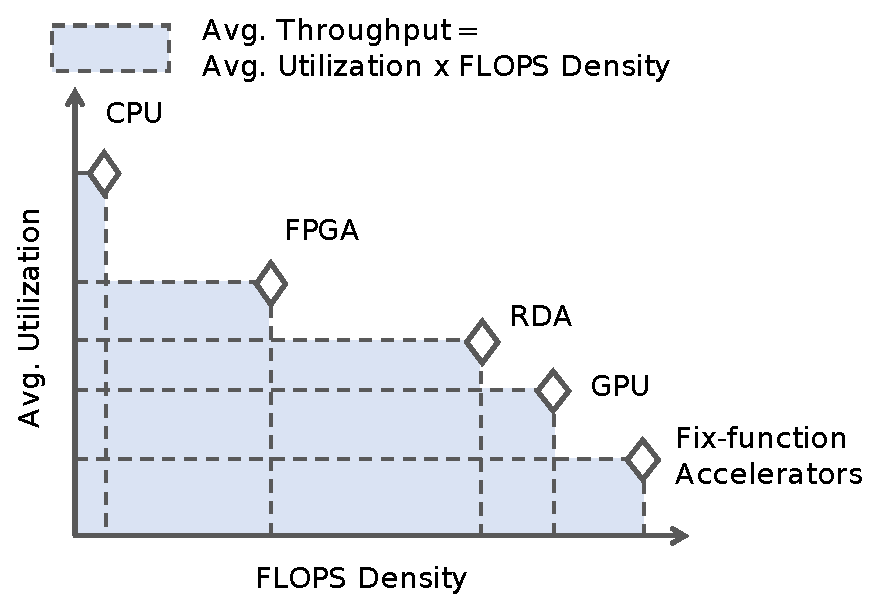
\includegraphics[width=0.4\textwidth]{figs/peakutil.pdf}
\caption[Average utilization vs. peak compute density tradeoff]{
 Tradeoff between the average utilization of the peak FLOPS over a range of applications vs. the peak compute density 
 among different architectures.
 The shaded area indicates the effective FLOPS achieved.
 With all the dynamic scheduling hardware in CPUs, such as prefetching and branch prediction, 
 CPU can achieve a fairly decent instruction per cycle (IPC) for data-analytic workloads that have a 
 regular control flow. 
 However, overheads to support flexibility, security, and programmability in CPU result in a low FLOPS
 density. 
 While GPU and fix-function accelerators have a high FLOPS density, they are prone to
 underutilization due to variation in application characteristics. 
 Fine-grained reconfigurable datapath makes it easy to utilize on-chip resources of an FPGA.
 However, the soft logics and overheads in routing resources lead to a low resource density and clock frequency.
 RDAs have the right balance between flexibility and efficiency, which gives a good overall average utilization.
}
\label{fig:peakutil}
\end{figure*}

Reconfigurable spatial architectures overcome this limitation by changing its datapath based on applications' needs.
Applications are configured at the circuit-level without dynamic instruction fetching and decoding,
hence improving energy-efficiency~\cite{calhoun,fpgaPower}.
In addition to instruction, data, and task-level parallelism explored by processor architectures, spatial architectures also explore instruction and task-level
pipelining that further increase the compute throughput~\cite{spatial-computation}.
Exploring pipeline parallelism enables spatial architectures to achieve a high-throughput
without massively parallelize every stage of the program.
Flexible datapath also permits resource distribution proportional to the compute intensity of
program stages.
A key performance optimization on reconfigurable accelerators is an application-level design space
exploration 
searching for the best resource distribution scheme that balances the compute pipeline~\cite{dse_koeplinger}.

One of the mainstream reconfigurable spatial architecture is 
Field Programmable Gate Arrays (FPGAs) that support fine-grain, 
bit-level reconfigurability with a soft logic fabric~\cite{fpga-survey}.
The flexible interconnect and lookup table-based logic gate can be configured to implement arbitrary
datapath.
FPGAs have been used to deploy services commercially~\cite{microsoft, baidu, deephi} and can be rented on the AWS F1 cloud~\cite{aws}. 
Although around for a long time, FPGAs are not broadly accepted among high-level application programmers due to their low-level programming interface and long compilation time.
Fine-tuning applications on FPGAs require expertise in digital design and takes a long
development cycle, which hinders their accessibility to the general software community.
As an application-level accelerator, FPGAs also suffers from overhead in fine-grained reconfigurability; 
studies have shown that over 60\% of the chip area of an FPGA is spent on routing resources~\cite{fpgaSurvey, calhoun, fpgaPower}. 

%Lately, Reconfigurable Dataflow Architecture (RDAs)~\cite{plasticine, ti, streamdataflow,neuflow,cnndataflow,dataflowarch} are emerging as a new class of spatial accelerators that 
%retain the desired level of flexibility and energy efficiency without 
%the area overhead and low clock frequency due to bit-level reconfigurability.
%As a subclass of Coarse-Grained Reconfigurable Arrays (CGRAs), RDAs also have
%coarse-grained building blocks, such as ALUs, register files, and memory controllers, 
%distributed in a programmable, word or vector-level static interconnect~\cite{adres, kress, dyser, 
%piperench, tartan, hrl, hycube}.

In contrast to fine-grained reconfigurable architectures,
Coarse-Grained Reconfigurable Arrays (CGRAs) are spatial architectures with 
coarse-grained building blocks, such as ALUs, register files, and memory controllers, 
distributed in a programmable, word or vector-level static interconnect~\cite{adres, kress, dyser, piperench, tartan, 
hrl, hycube}.
We refer a subclass of CGRAs with dataflow-driven execution model as Reconfigurable Dataflow
Architectures (RDAs)\footnote{Dataflow overlay architectures on FPGA are technically also RDAs, which are not the primary concern in the discussion of this work.}~\cite{plasticine, ti, streamdataflow,neuflow,cnndataflow,dataflowarch}.
Lately, RDAs are emerging as a new class of spatial accelerators that retain the desired level of
flexibility and energy efficiency without the area overhead and low clock frequency of bit-level reconfigurability.
Our previously proposed RDA--Plasticine--has demonstrated a promising acceleration of dense, sparse, database, and streaming applications~~\cite{plasticine, gorgon, multijoin,prabhakarthesis}.
To meet the computing demand of recent data-analytic workload, Plasticine is a large-scale RDA
compared to traditional CGRAs. 
\Cref{tab:ops} shows the OPS comparison across a few CGRAs proposed in the prior works.

\begin{table}
  \centering
\begin{tabular*}{0.88\textwidth}{cccccc}
  \toprule
  \textbf{Architectures} & DySER~\cite{dyser} & TI~\cite{ti} & revel~\cite{revel}
  & Plasticine~\cite{plasticine} & Gorgon~\cite{gorgon}\\\midrule
  \textbf{OPS} & 128GOPS & 64GOPS & 300GOPS & 12.3TFLOPS & 38.4TFLOPS \\
  \bottomrule
\end{tabular*}
\caption[OPS comparison of different CGRAs]{OPS comparison of different CGRAs. Gorgon is a
Plasticine variant proposed for joint machine learning and database acceleration.}
\label{tab:ops}
\end{table}

The scale of Plasticine introduces challenges in network-on-chip design to sustain 
bandwidth requirements while staying energy-efficient.
On the other hand, we also need to adjust the compilation strategy to explore multiple-levels of
concurrency in the program to saturate the compute throughput of the large-scale RDA;
this strategy must introduce minimum synchronization overhead to maximize the scalability of the mapped design.

\section{The Need for Flexible Interconnects}
Applications are mapped to RDAs by distributing computations spatially across multiple processing
blocks and executing them in a pipelined, data-driven fashion. 
On traditional Networks on Chip
(NoCs) for multicore systems, communication is the result of explicit message passing between
parallel workers or messages to handle cache misses from the coherence protocol; these are bursty and
relatively infrequent. 
On RDAs, however, applications are distributed by parallelizing and pipelining; 
pipelining introduces frequent and throughput-sensitive communication. 
Because different applications are parallelized and pipelined differently, they have different communication requirements.

\begin{figure*}
\centering
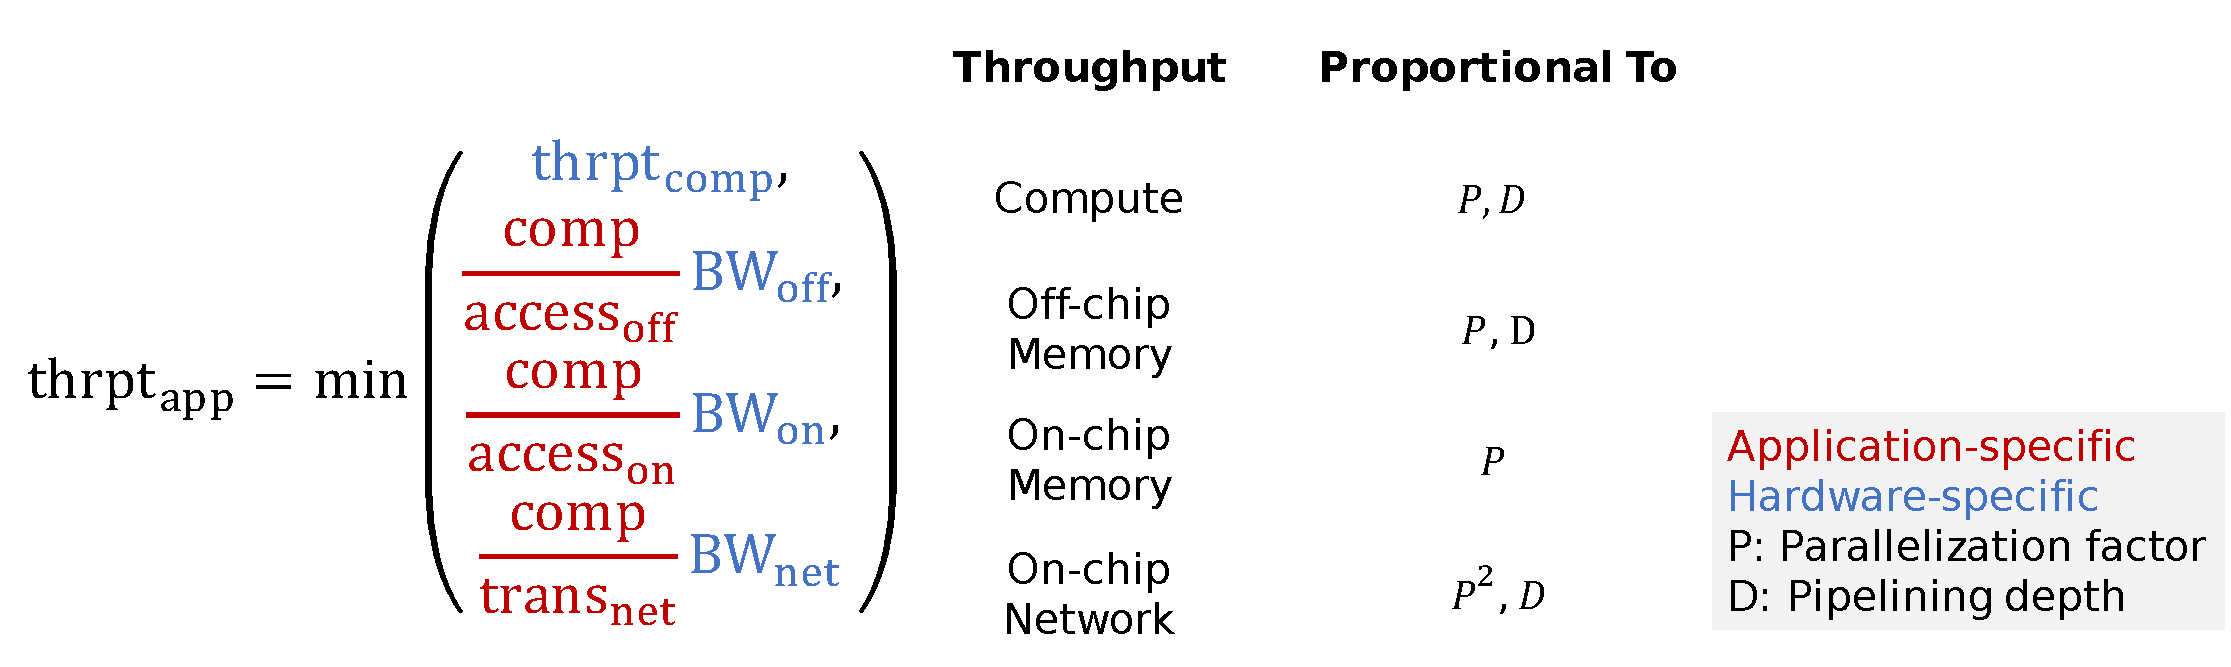
\includegraphics[width=1\textwidth]{figs/perfmodel.pdf}
\caption[High-level performance model of a spatial architecture]{
High-level performance model of a spatial architecture. 
}
\label{fig:perfmodel}
\end{figure*}

\Cref{fig:perfmodel} shows a high-level performance model of a spatially pipelined and parallelized
reconfigurable architecture.
Due to pipelined execution, the performance of a spatial architecture is dominant by throughput as
supposed to latency. 
Compute, on and off-chip memory accesses, and network become a integrated pipeline, 
where performance is limited by the pipeline stage with lowest throughput.
The red terms in the equation are application-specific and capture the compute, memory, or IO-bound characteristics.
The blue terms are the available bandwidth and FLOPS on the hardware.
While the compute and memory access in application increases linearly with parallelization factor and pipelining depth,
the required network bandwidth from application increases quadratically with increasing parallelism.
This means as we going to larger chip size, the network bandwidth must grow super linearly in
order to achieve a perfect performance scaling, unless exploring pipeline parallelism.

RDAs need the right amount of interconnect flexibility to achieve good resource utilization; 
an inflexible interconnect constrains the space of
valid application mappings and hinders resource utilization. 
Furthermore, 
in the quest to increase compute density, RDA data paths now 
contain increasingly coarse-grained processing blocks such as pipelined, vectorized functional 
units~\cite{plasticine, piperench, xilinx-acap}.
Plasticine, as an example, has a 512-bit vector bus, which necessitates coarser communication and higher on-chip interconnect bandwidth to avoid creating performance bottlenecks. 
Although many hardware accelerators with large, vectorized data paths have fixed local networks~\cite{brainwave}, there is a need for more
flexible global networks to adapt to future applications.
Consequently, interconnect design for these RDAs involves achieving a balance between the often conflicting requirements of high bandwidth and high flexibility.

\section{The Gap between High-Level DSLs and Dataflow Accelerators}

\begin{figure*}
\centering
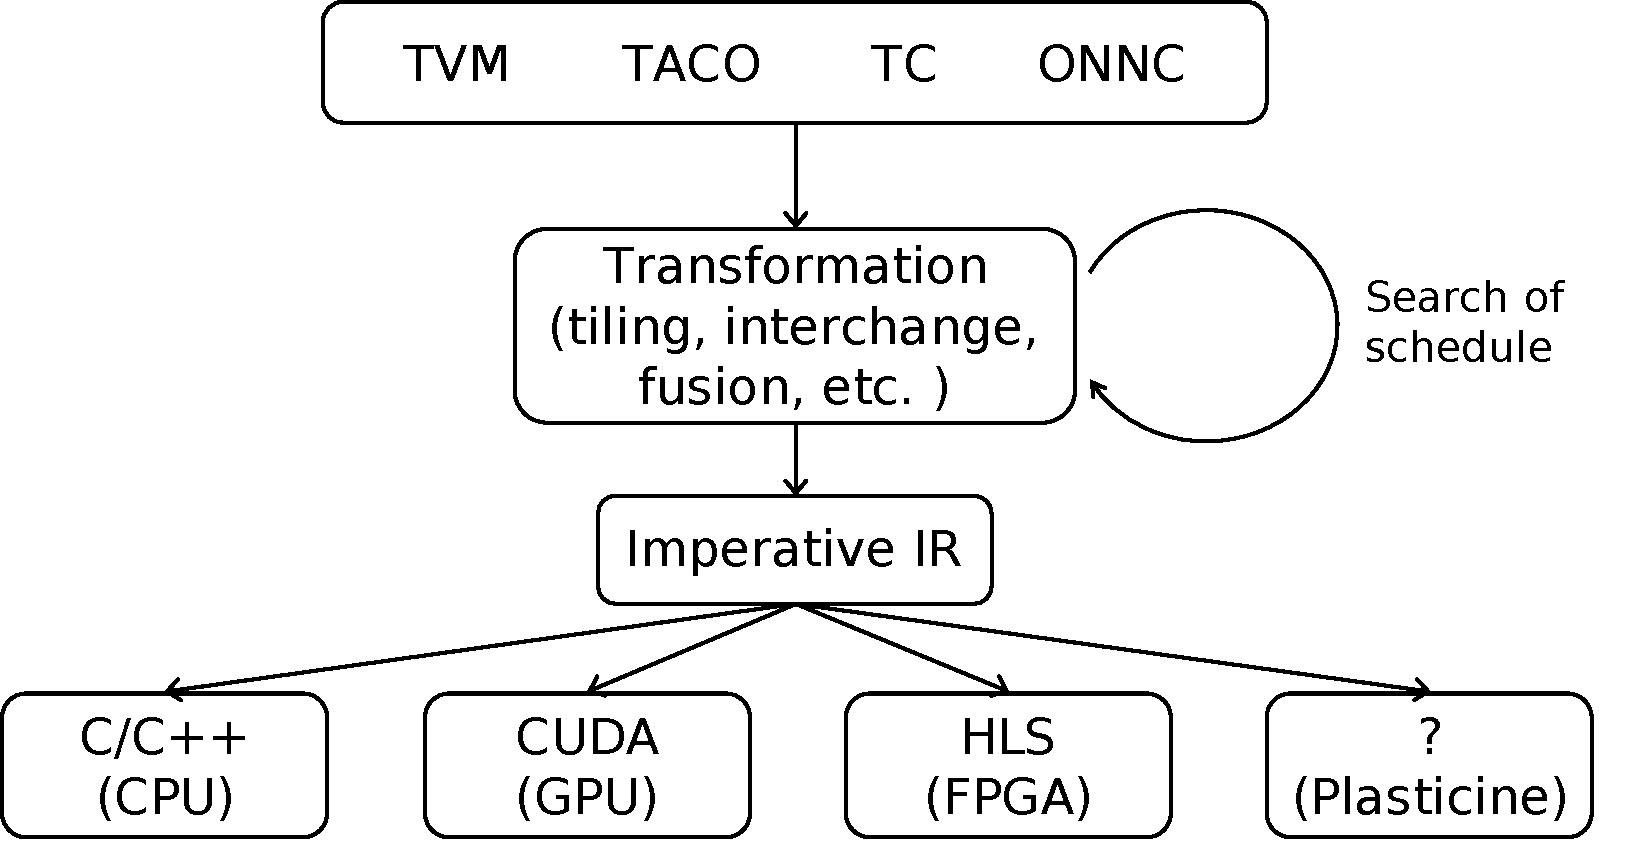
\includegraphics[width=0.6\textwidth]{figs/highlevel.pdf}
\caption[Big picture of accelerator compiler stack]{
  Big picture of accelerator compiler stack.
}
\label{fig:bigpic}
\end{figure*}

Recent years have seen a rise in interests in hardware accelerators, primarily motivated by AI applications. 
Research in software infrastructure for these accelerators, however, is just emerging.
Unlike CPUs, these accelerators do not support a standard ISAs, alleviating the overhead from
layers of abstractions and the burden of backward compatibility. 
Nonetheless, lack of a common abstraction makes it very hard to sharing compiler infrastructure
across accelerators. 

\section{Contribution}

In this work, we start by detailing the key considerations involved in building an RDA network, including those arising from network design, RDA architecture, and the characteristics of spatially mapped applications.
Network designs must be carefully considered because vectorization magnifies inefficiencies: the increased network area of a vectorized design ensures that any overhead has a significant impact.
Next, we evaluate the performance, area, and power requirements of several interconnection designs using cycle-accurate simulation and ASIC synthesis of a switch and router with a \SI{28}{nm} industrial technology library.
We then explore a variety of design points, including static, dynamic, and hybrid networks, decreased flit widths and VC counts for dynamic networks and different flow-control strategies for static networks.

We show that RDA network designs must consider application characteristics and the execution model of the underlying architecture.
Performance scales strongly with network bandwidth, with an 8x average performance gap between the best and worst configurations. 
The hybrid network gives the best network energy-efficiency: a 1.83x average improvement over the static network. On pipelined architectures,
hybrid networks can also match the performance per area of higher bandwidth, purely static networks with less than 8\% performance loss.

The key contributions of this paper are:
\begin{enumerate}
    \item An analysis of key communication patterns exhibited by spatial architectures.
    \item A network-aware compiler flow that efficiently targets static, dynamic, and hybrid networks with varying granularities.
    \item A quantitative analysis of the performance, area, and energy trade-offs involved in choosing an RDA network, using benchmarks drawn from various application domains.
\end{enumerate}

\section{Outline}

  \chapter{Background (WIP)}

\section{Execution Schedules of Reconfigurable Architectures} 
\begin{figure*}
\begin{subfigure}[b]{0.34\textwidth}
\inputminted{python}{code/spatialeg2.py}
\caption {
}
\end{subfigure}
\hfill
\begin{subfigure}[b]{0.65\textwidth}
\centering
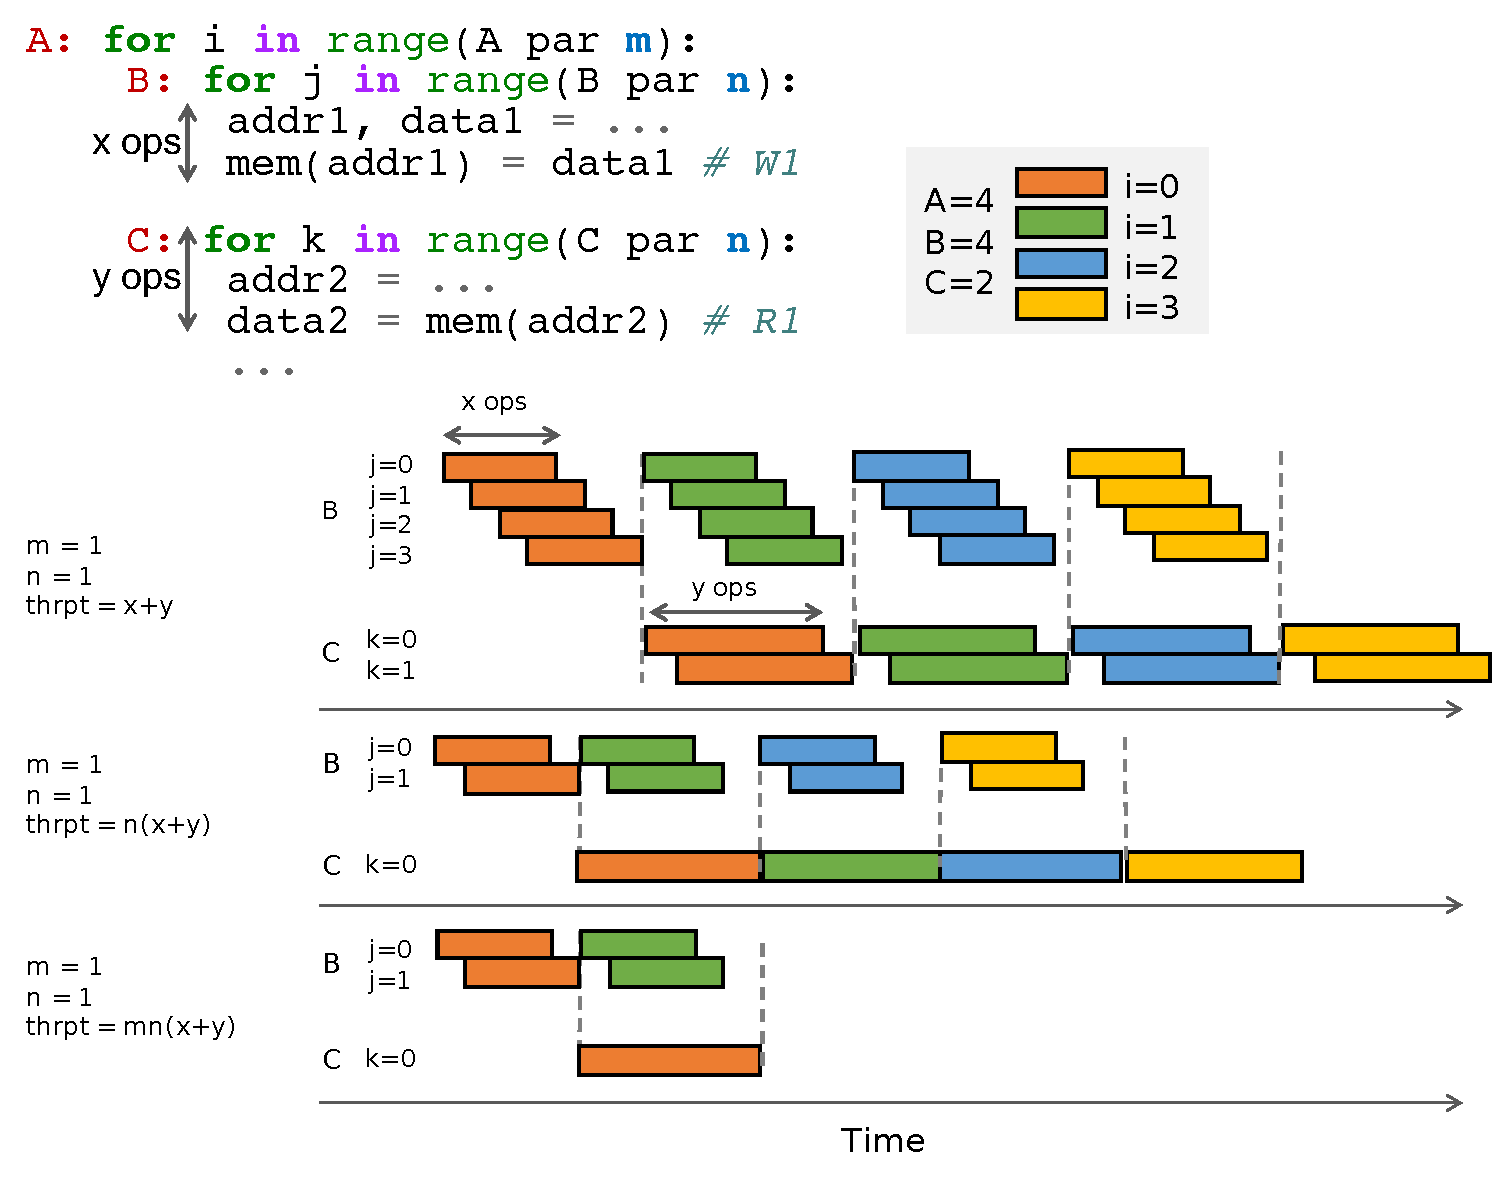
\includegraphics[width=1.0\textwidth]{figs/pipeexec.pdf}
\caption {
}
\end{subfigure}
\caption[Hiearchical pipelining and parallelization on spatial architecture]{
Hierarchical pipelining and parallelization in spatial architecture.
(a) illustrates the runtime and throughput of a hierarchically pipelined and parallelized program on
a reconfigurable spatial architecture. 
At inner level, instructions within each basic
block are fine-grained pipelined across iterations of the inner most loop. 
At outer level, the inner loops are coarse-grained pipelined across the outer loop iterations.
Exploiting multiple levels of pipeline parallelism gives a total throughput of $x+y$ operations per
  cycle, where \emph{x} and \emph{y} are number of operations in the basic blocks.
(b) Vectorizing the inner most loops B and C by \texttt{n} increases the throughput to $(x+y)n$.
(c) Parallelizing the outer loop A by \texttt{m} further increases the throughput to $(x+y)mn$.
}
\label{fig:pipeexec}
\end{figure*}

\begin{figure*}
\centering
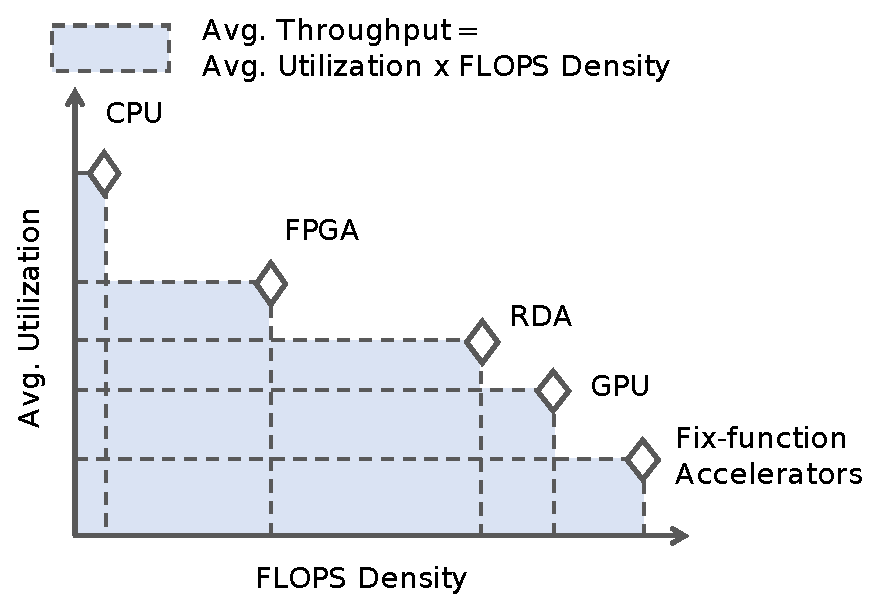
\includegraphics[width=0.4\textwidth]{figs/peakutil.pdf}
\caption[Average utilization vs. peak compute density tradeoff]{
 Average utilization vs. peak compute density tradeoff among different architectures.
}
\label{fig:peakutil}
\end{figure*}

\begin{figure*}
\centering
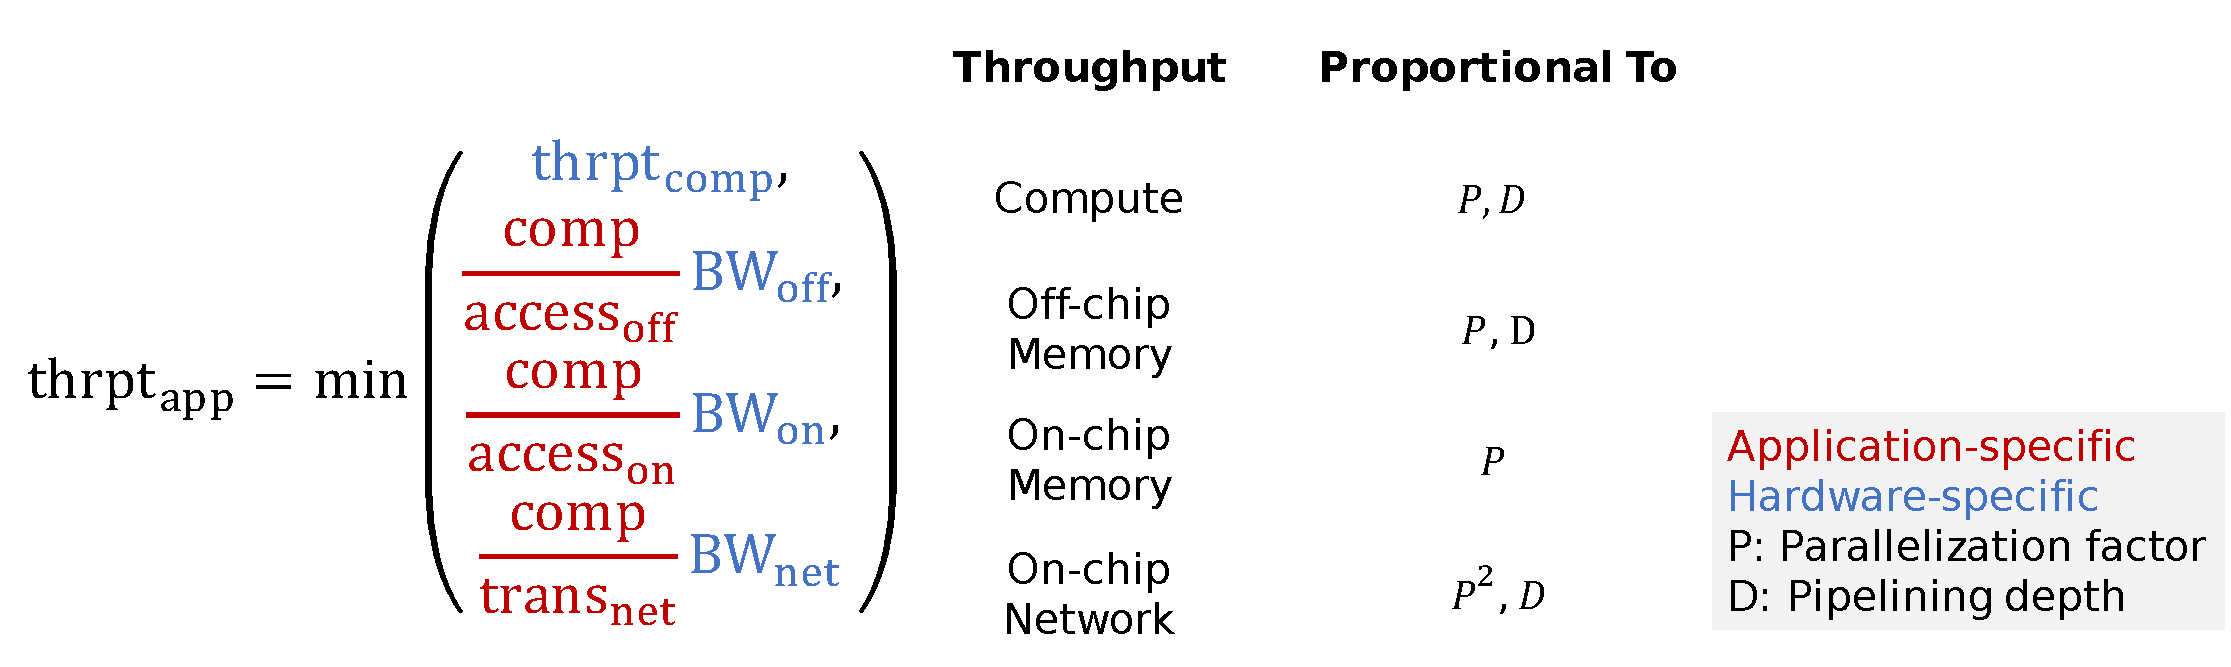
\includegraphics[width=1\textwidth]{figs/perfmodel.pdf}
\caption[High-level performance model of spatial architectures]{
High-level performance model of spatial architectures
}
\label{fig:perfmodel}
\end{figure*}

The key advantage of reconfigurable spatial accelerators, compared to processor-based architectures, 
is the ability to explore multiple levels of pipeline parallelism. 
In traditional Von Neumann architectures~\cite{vonneumann}, like CPUs and GPUs,
a computer consists of a processing unit that performs
computation, a memory unit that stores the program states, and a control unit that tracks execution
states and fetch the instruction to execute. This computing model inherently assumes that
instructions with in a program are executed in time, maximizing the flexibility to 
context switching between different workloads dynamically.

Reconfigurable accelerators are a direct violation of the von Neumann execution model; 
instructions are statically imbedded in the datapath and executed in space as supposed to in time.
One of the disadvantage of reconfigurable hardware is paying the resource cost for infrequently
executed instructions, making it unsuitable for control-heavy workloads that traditional
processors are efficient at.
On the other hand, RDAs are particularly competitive in providing high-throughput, 
low-latency, and energy-efficiency acceleration for data-analytical workloads.
Data-analytical workloads encompass a wide domains of applications, including image processing,
recognition, machine translation, digital signal processing, network processing, etc.
These applications exhibits a rich amount of data-level parallelism with relatively static control
flow.

\Cref{fig:pipeexec} shows an example of hierarchical parallelism and pipelining exploit by
a spatial architecture.
The overall compute throughput of a parallelized and pipelined program is 
the product of the total parallelization factors and pipelining depth.
By exploring multiple dimensions of concurrency in the program, spatial architecture is more likely
to achieve a good compute throughput for a wide range of applications.
For applications that are expensive to parallelize due to irregular access patterns, spatial
architectures can increase on the pipelining dimension;
for application with embarrassingly parallel workloads, spatial architecture can budget most
resource on increasing parallelism.

Another benefit of pipelined execution is easier to achieve good memory performance.
Data accessed by different stage of the pipelines are stored in discrete scratchpads 
instead of a shared cache; improving the effective on-chip bandwidth and capacity.
Using explicitly managed scratchpad also tends to improve locality and 
eliminate cache performance issues, such thrashing.
Across kernels, pipelined execution reduces the amount of off-chip accesses for intermediate
data.
SIMT architectures, like GPUs, relying on high-bandwidth DRAM technology, such has HBM, to sustain
the compute throughput of massively parallelized threads.
While providing over 10x more bandwidth than traditional DDR technologies, HBM is very limited in
capacity, around 16GB as supposed to on the orders of TB for DDR.
As a result, the limited off-chip capacity often restricts the type of applications that
GPUs can support.

%\begin{table*}
  %\centering
%\begin{tabular}{lccc}
  %\toprule
 %Concurrency Level & Instruction & Data & Task/Kernel  \\ \midrule
 %Parallelsim & CPU,\rda & CPU,GPU,\rda & CPU,\rda  \\
 %Pipelining & \rda & \rda & \rda \\
 %\bottomrule
%\end{tabular}
%\caption[Concurrency level explored by different architectures]{
  %Concurrency level explored by different architectures
%}
%\label{tab:conclevel}
%\end{table*}


  \section{RNN Computation Analysis} 
\label{sec:app}
In this section, we first discuss the limitation of BLAS-based LSTM on processor and spatial architectures.
Next, we discuss our implementation of loop-based LSTM on spatial architectures.
Table \ref{tab:legend_app} contains specifications for symbols and parameters
  used in this section.
\begin{table}[t]
  \vskip 0.15in
  \centering
  \scriptsize
  \begin{tabular}{p{0.6cm}m{3cm}m{3cm}}
  \toprule
    Symbol & Processor & Reconfigurable Hardware \\
    \midrule
    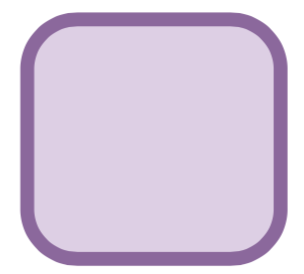
\includegraphics[width=0.03\columnwidth]{figs/innerloop.png} & Kernel & Inner Loop \\
    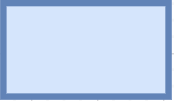
\includegraphics[width=0.03\columnwidth]{figs/onchip.png} & Memory Hiearchy & On-chip Scratchpad \\
    
\includegraphics[width=0.03\columnwidth]{figs/reg.png} & Register File & Register \\
    
\includegraphics[width=0.1\columnwidth]{figs/unrollparm.png} & & Unrolling factor using multiple hardware compute blocks \\ \midrule
    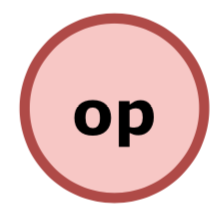
\includegraphics[width=0.03\columnwidth]{figs/vec.png} & \multicolumn{2}{L{6.5cm}}{Element-wise Operation} \\
    
\includegraphics[width=0.03\columnwidth]{figs/outerloop.png} & \multicolumn{2}{L{6.5cm}}{Outer Loop} \\
    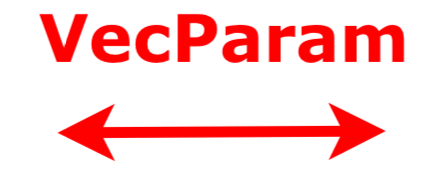
\includegraphics[width=0.1\columnwidth]{figs/vecparam.png} & \multicolumn{2}{L{6.5cm}}{Vectorization parameter for AVX or SIMD instructions} \\
    \midrule
    \midrule
    Parameter & \multicolumn{2}{l}{Specification} \\
    \midrule
    $hv$      & \multicolumn{2}{l}{Vectorization parameter on H} \\
    $hu$      & \multicolumn{2}{l}{Unrolling factor on H} \\
    $rv$      & \multicolumn{2}{l}{Vectorization parameter on R} \\
    $ru$      & \multicolumn{2}{l}{Unrolling factor on R} \\
    $G$       & \multicolumn{2}{l}{Number of gates in an RNN. For LSTM, G=4} \\
  \bottomrule
  \end{tabular}
  \caption{Specifications for symbols and parameters in Section \ref{sec:app}.}
  \label{tab:legend_app}
  \vskip -0.1in
  \end{table}

\begin{figure*}
  \centering
  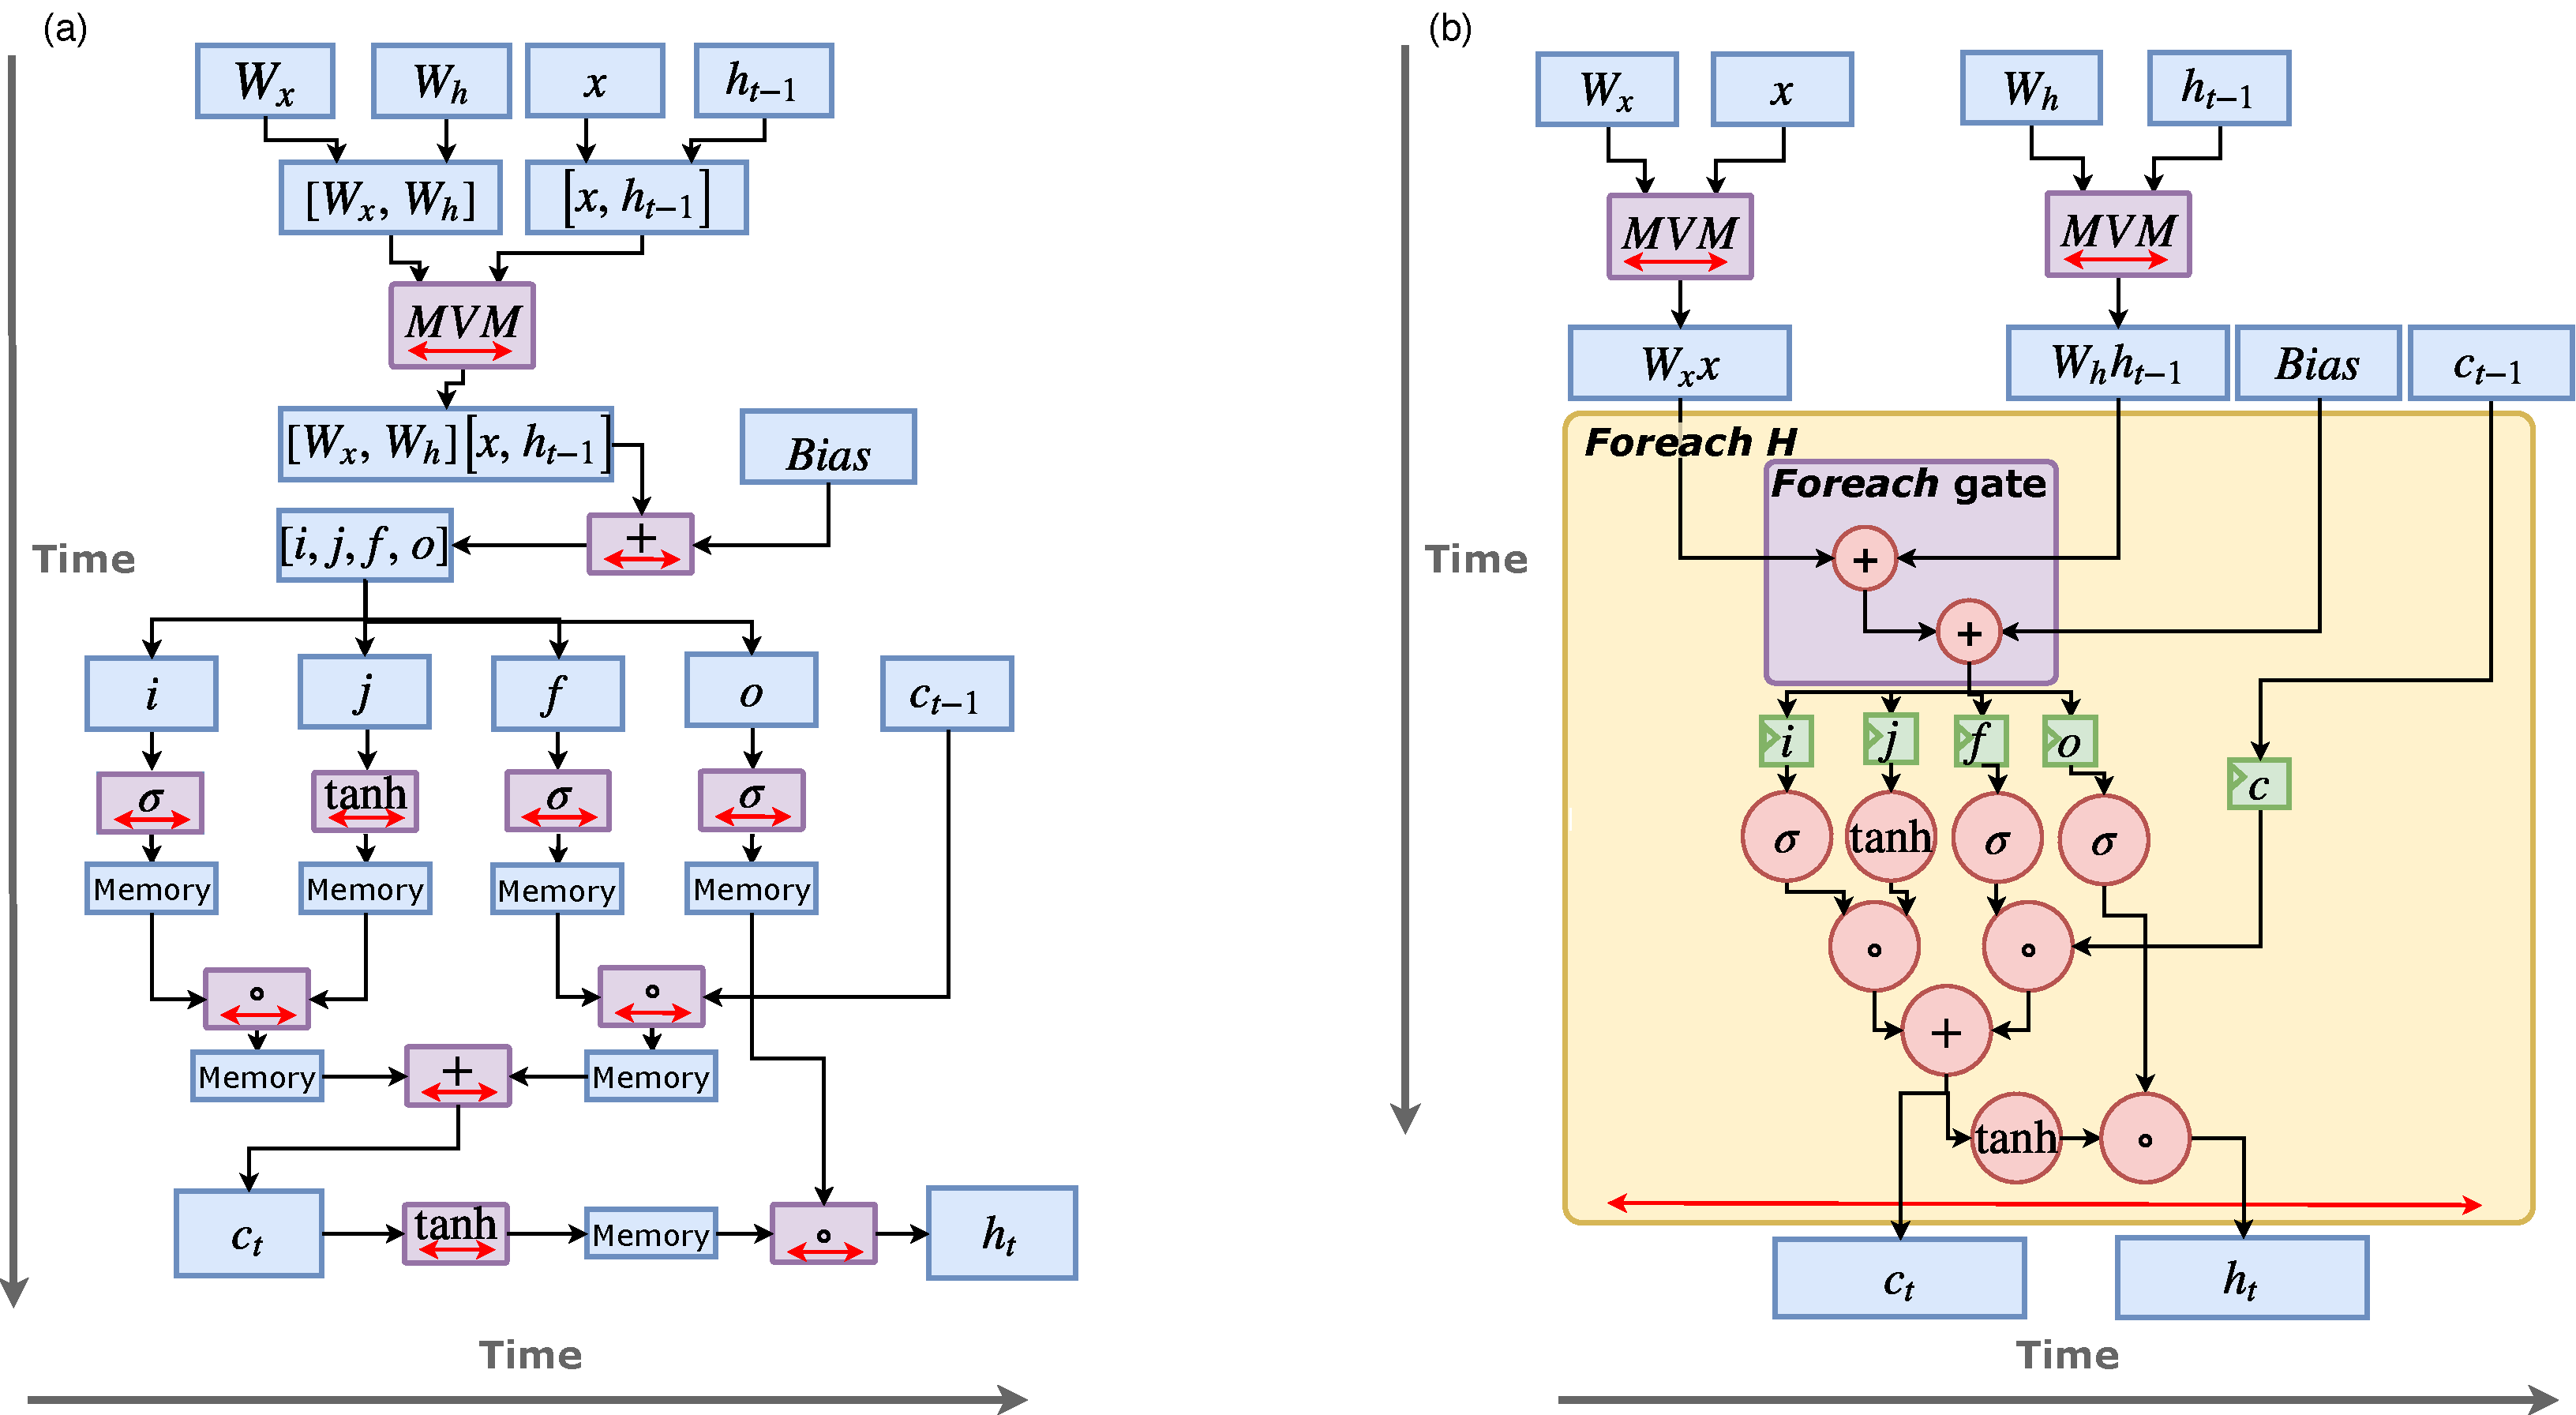
\includegraphics[width=1.5\columnwidth]{figs/cpugpulstm.pdf}
  \caption{Compute and memory layout of TensorFlow \texttt{BasicLSTM} cell on CPU (a) and \texttt{CudnnLSTM} cell on GPU (b).}\label{fig:tf_lstm}
\end{figure*}

\subsection{BLAS-based LSTM on Processor Architecture}
Modern Machine Learning frameworks, e.g.
  TensorFlow \cite{abadi2016tensorflow},
  divide the computation graph of an LSTM cell into BLAS kernels.
Then, the BLAS kernel is accelerated by calling low-level
optimized BLAS subroutines such as Intel BLAS Library on CPU
and NVBLAS Library on GPU.
Figure \ref{fig:tf_lstm} (a) shows the computation graph of a \texttt{BasicLSTM} cell in TensorFlow.
This implementation can lead to large memory footprint since all the intermediate results are
  materialized in memory.
A common strategy to tackle the issue is through fusing blocked kernels.
With TensorFlow's abstraction, this can only be achieved by
  expressing the entire RNN cell as an optimized kernel.
For example, TensorFlow provides \texttt{LSTMBlockFusedCell} and \texttt{GRUBlockCell} modules,
  which are the fastest TensorFlow implementations of RNN cells for CPU.
In practice, such implementation can provide significant performance improvement
  over the \texttt{BasicLSTM} implementation.
However, it is still very hard to saturate CPU compute capacity, potentially
due to the high synchronization overhead across threads.
Figure \ref{fig:tf_lstm} (b) shows the computation layout of TensorFlow with
cuDNN library \cite{chetlur2014cudnn} on GPU. cuDNN is an NVIDIA GPU
library for accelerating deep neural networks.
To minimize the data movement,
  cuDNN fuses all the vector-vector (VV) operations after MVM. Specifically, the bias add in
  Equation \ref{eq:1}, \ref{eq:2}, \ref{eq:3}, \ref{eq:4},
  and all the operations in Equation \ref{eq:5}, \ref{eq:6},
  are fused into one kernel.
Nevertheless, there are still intermediate buffers of size $H$
  between the MVM kernel and the element-wise operations.

Compared to the \texttt{BasicLSTM} implementation,
  \texttt{CudnnLSTM} eliminates most of large intermediate memories.
However, the MVMs of Equation \ref{eq:1}, \ref{eq:2}, \ref{eq:3}, \ref{eq:4} are all accelerated
with BLAS3 kernels, which performs only matrix-matrix level operations.
This turns MVM and VV bias add into Matrix Matrix Multiplication (MMM) and Matrix Matrix
Addition (MMA), which leads to serious underutilization of GPU.

Moreover, a processor-based architecture introduces large energy overhead of instruction
  decoding and scheduling.
GPU especially suffers from its power-hungry, high-throughput memory hierarchy.
For these reasons, both the CPU and GPU architectures are not suitable
  for energy-efficient, low-latency RNNs serving platforms.

\subsection{BLAS-based LSTM on Spatial Architecture}

Previous work has studied the capability of using an FPGA as a low-latency serving platform.
An FPGA has the flexibility of resizing MVM and VV units based on the application size.
In addition, MVM and VV units can be implemented with hardware pipelines,
  which removes the instruction scheduling and control overhead on a processor-based
  architecture.
The latest version of Intel Stratix 10 FPGA further boosts the compute power of FPGA
  with increasing number of hardened digital signal processing (DSP) blocks
  and on-chip memory capacity.
Microsoft Brainwave (BW) \cite{fowers2018configurable}
  is a state-of-the-art FPGA-based deep learning framework.

Figure \ref{fig:bw_lstm} shows BW's compute and memory layout.
In contrast to the CPU and GPU implementations, BW blocks the MVM along both
  row and column dimensions.
It then fuses the inner tiled MVM with element-wise non-linear functions.
Specifically for a matrix of size $H\times R$ and a vector of size $R$,
BW parallelizes the compute of multiple column tiles ($ru$, \# MV Tiles in the original paper) of size
$hv\times rv$ with multiple tiled engines, as shown in Figure \ref{fig:bwt} (a). 
Each tile engine contains $hv$ (native dimension) number of dot
product engines vectorized by $rv$ (lanes) and achieves one tile per cycle throughput. 
Parallel tiles along the row dimension are then fed into a pipelined reduction and accumulation
unit.
Immediately after the accumulation, the multi-function units (MFUs) execute the
element-wise operations on the $hv$ vector chunk produced by the accumulator.
Although BW's implementation still keeps the vectorized intermediate results, the size $hv$ is much
smaller than $H$ in \texttt{BasicLSTM} cell.
Nonetheless, with parallelization in $ru$,
  BW allocates lots of vectorized intermediate buffers that can still lead to energy inefficiency.
BW performs one MVM operation in $\ceil[\big]{\frac{H}{hv}}\ceil[\big]{\frac{R}{rv\cdot ru}}$
  iterations.

The MVM operations are executed on each gate of the LSTM sequentially.
Similarly, element-wise operations $hv$ using $\sigma, \tanh, \circ, +$ for the non-linear 
operators are also scheduled to execute on the vectorized multi-function units with size
of $hv$, as shown with the arrow in time in Figure \ref{fig:bw_lstm}.
To avoid DRAM communication overhead and improve compute density, Brainwave embeds MVM in a blocked floating-point format, 
where the vector of $hv$ values share a single 5-bit exponent and have distinct signs and 2-5 bit mantissa for
each value. As a result, they can achieve very dense low-precision compute and storage, with one
adder per $hv$ values and $hv$ multipliers for a vector of $hv$. The remaining operations are
performed in 16-bit precision.

When matrix dimensions cannot be divided by $hv$ and $rv\cdot ru$, Brainwave suffers from
underutilization of the compute FLOPS, as shown in Figure \ref{fig:bwt} (a).
The underutilization is worse with small problem sizes.
In addition, BW computes $W_xX$ and $W_hH$ separately rather than computing them with concatenated larger matrices,
  which can further aggravate the problem.
This might be because BW's abstraction does not allow partial updates of an vector
  but only $X$ is updated at the end of the step.


\subsection{Loop-based LSTM}
We have made the following observations
  from analyzing BLAS-based LSTM implementations:
\begin{enumerate}
\item 
  Constructing an LSTM cell's computation graph using BLAS subroutines
  introduces large intermediate buffers even when the kernels themselves are blocked.
  Each element on RNN cells' non-reduction dimension of the MVM ($H$)
  can be computed completely independently within one time step. This
  exposes the opportunity of fine-grain loop tiling and fusion across the
  entire LSTM kernel. 
\item MVM is the computation bottleneck in serving RNN cells. Spatial
  architecture allows us to distribute most of the compute resource to MVM 
  by parallelizing and pipelining MVM with element-wise operations.
\item Using low-precision operations can boost compute density and keep RNN
  weights on-chip to avoid high-latency DRAM communication. We need to introduce
  efficient low-precision support in the target spatial architecture without introduce
  too much overhead.
\end{enumerate}

To address the issue of large intermediate buffers, we fine-grain tile and fuse
MVM with non-linear functions. We refer to the computation for generating 
every single element in $c_t$ and $h_t$ as LSTM-1 operation, which can be computed
independently in a single step. LSTM-1 is composed of four independent dot products of 
the row vectors of the weight matrices with the input vector immediately followed by the 
element-wise operations on output of the dot product. The resulting $c$ and $t$ vectors are 
produced by computing LSTM-1 operations for $H+D$ iterations.

\label{sec:blaslstm}
 \begin{figure}
  \centering
  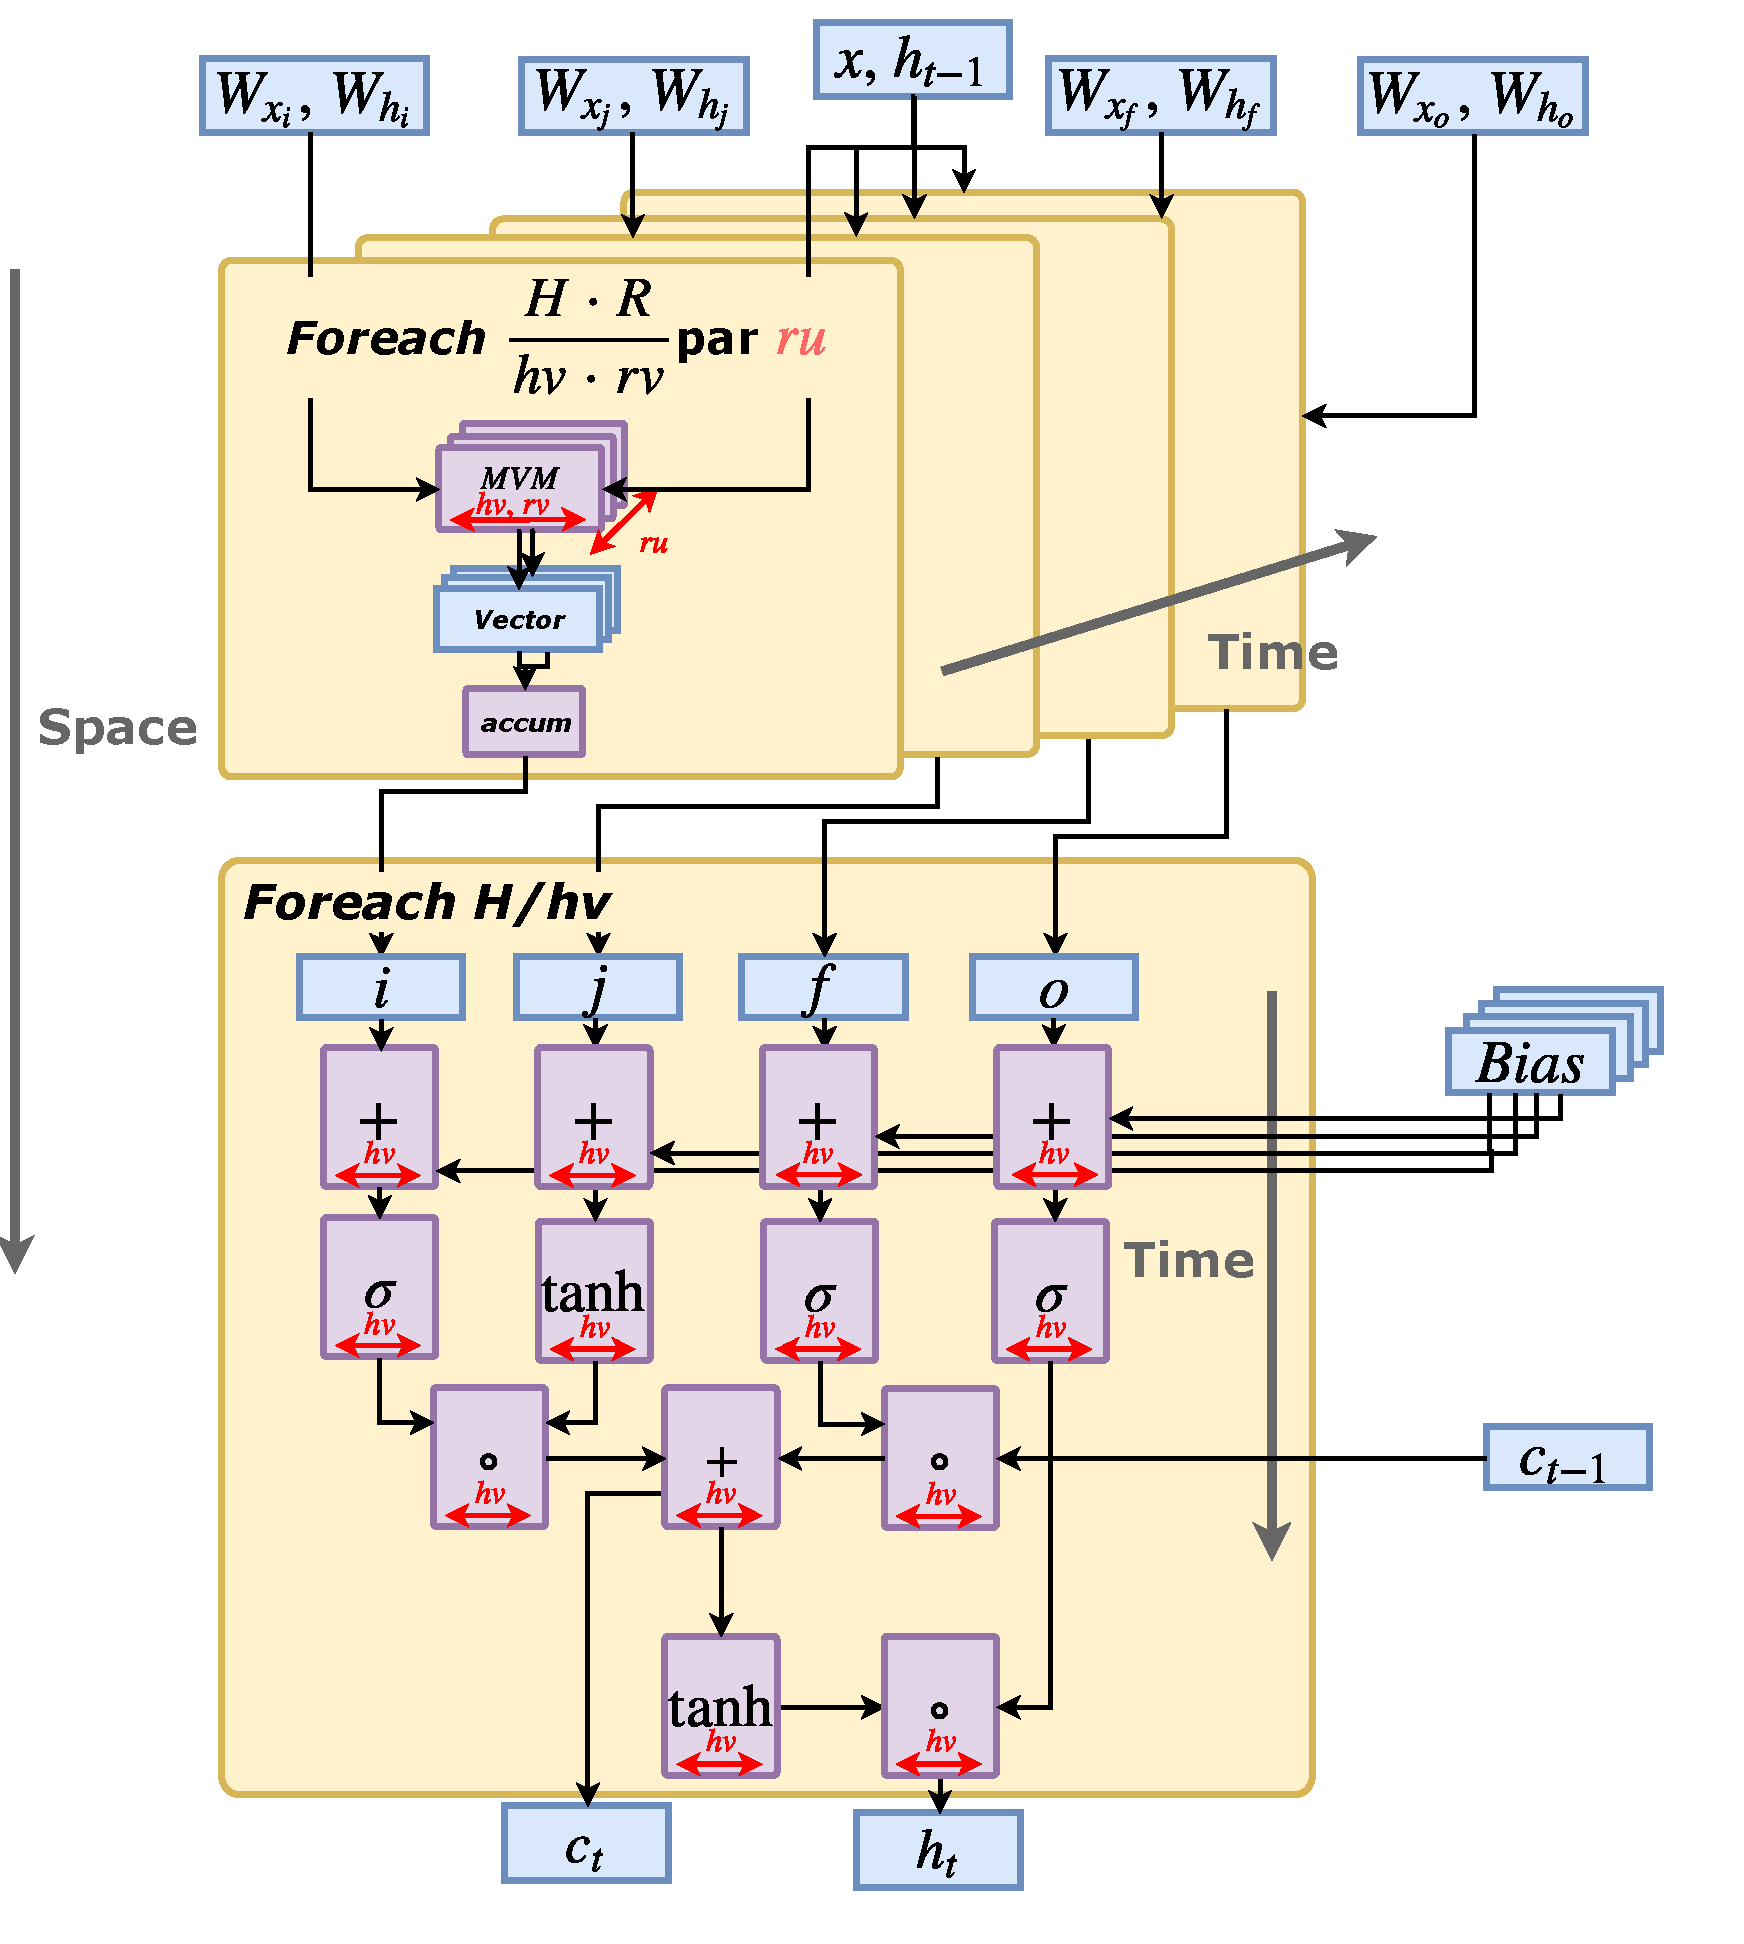
\includegraphics[width=0.8\columnwidth]{figs/bwlstm.pdf}
  \caption{Compute and memory layout of LSTM in Brainwave.}\label{fig:bw_lstm}
   \vspace*{-0.3in}
\end{figure}

\begin{figure}
 \centering
  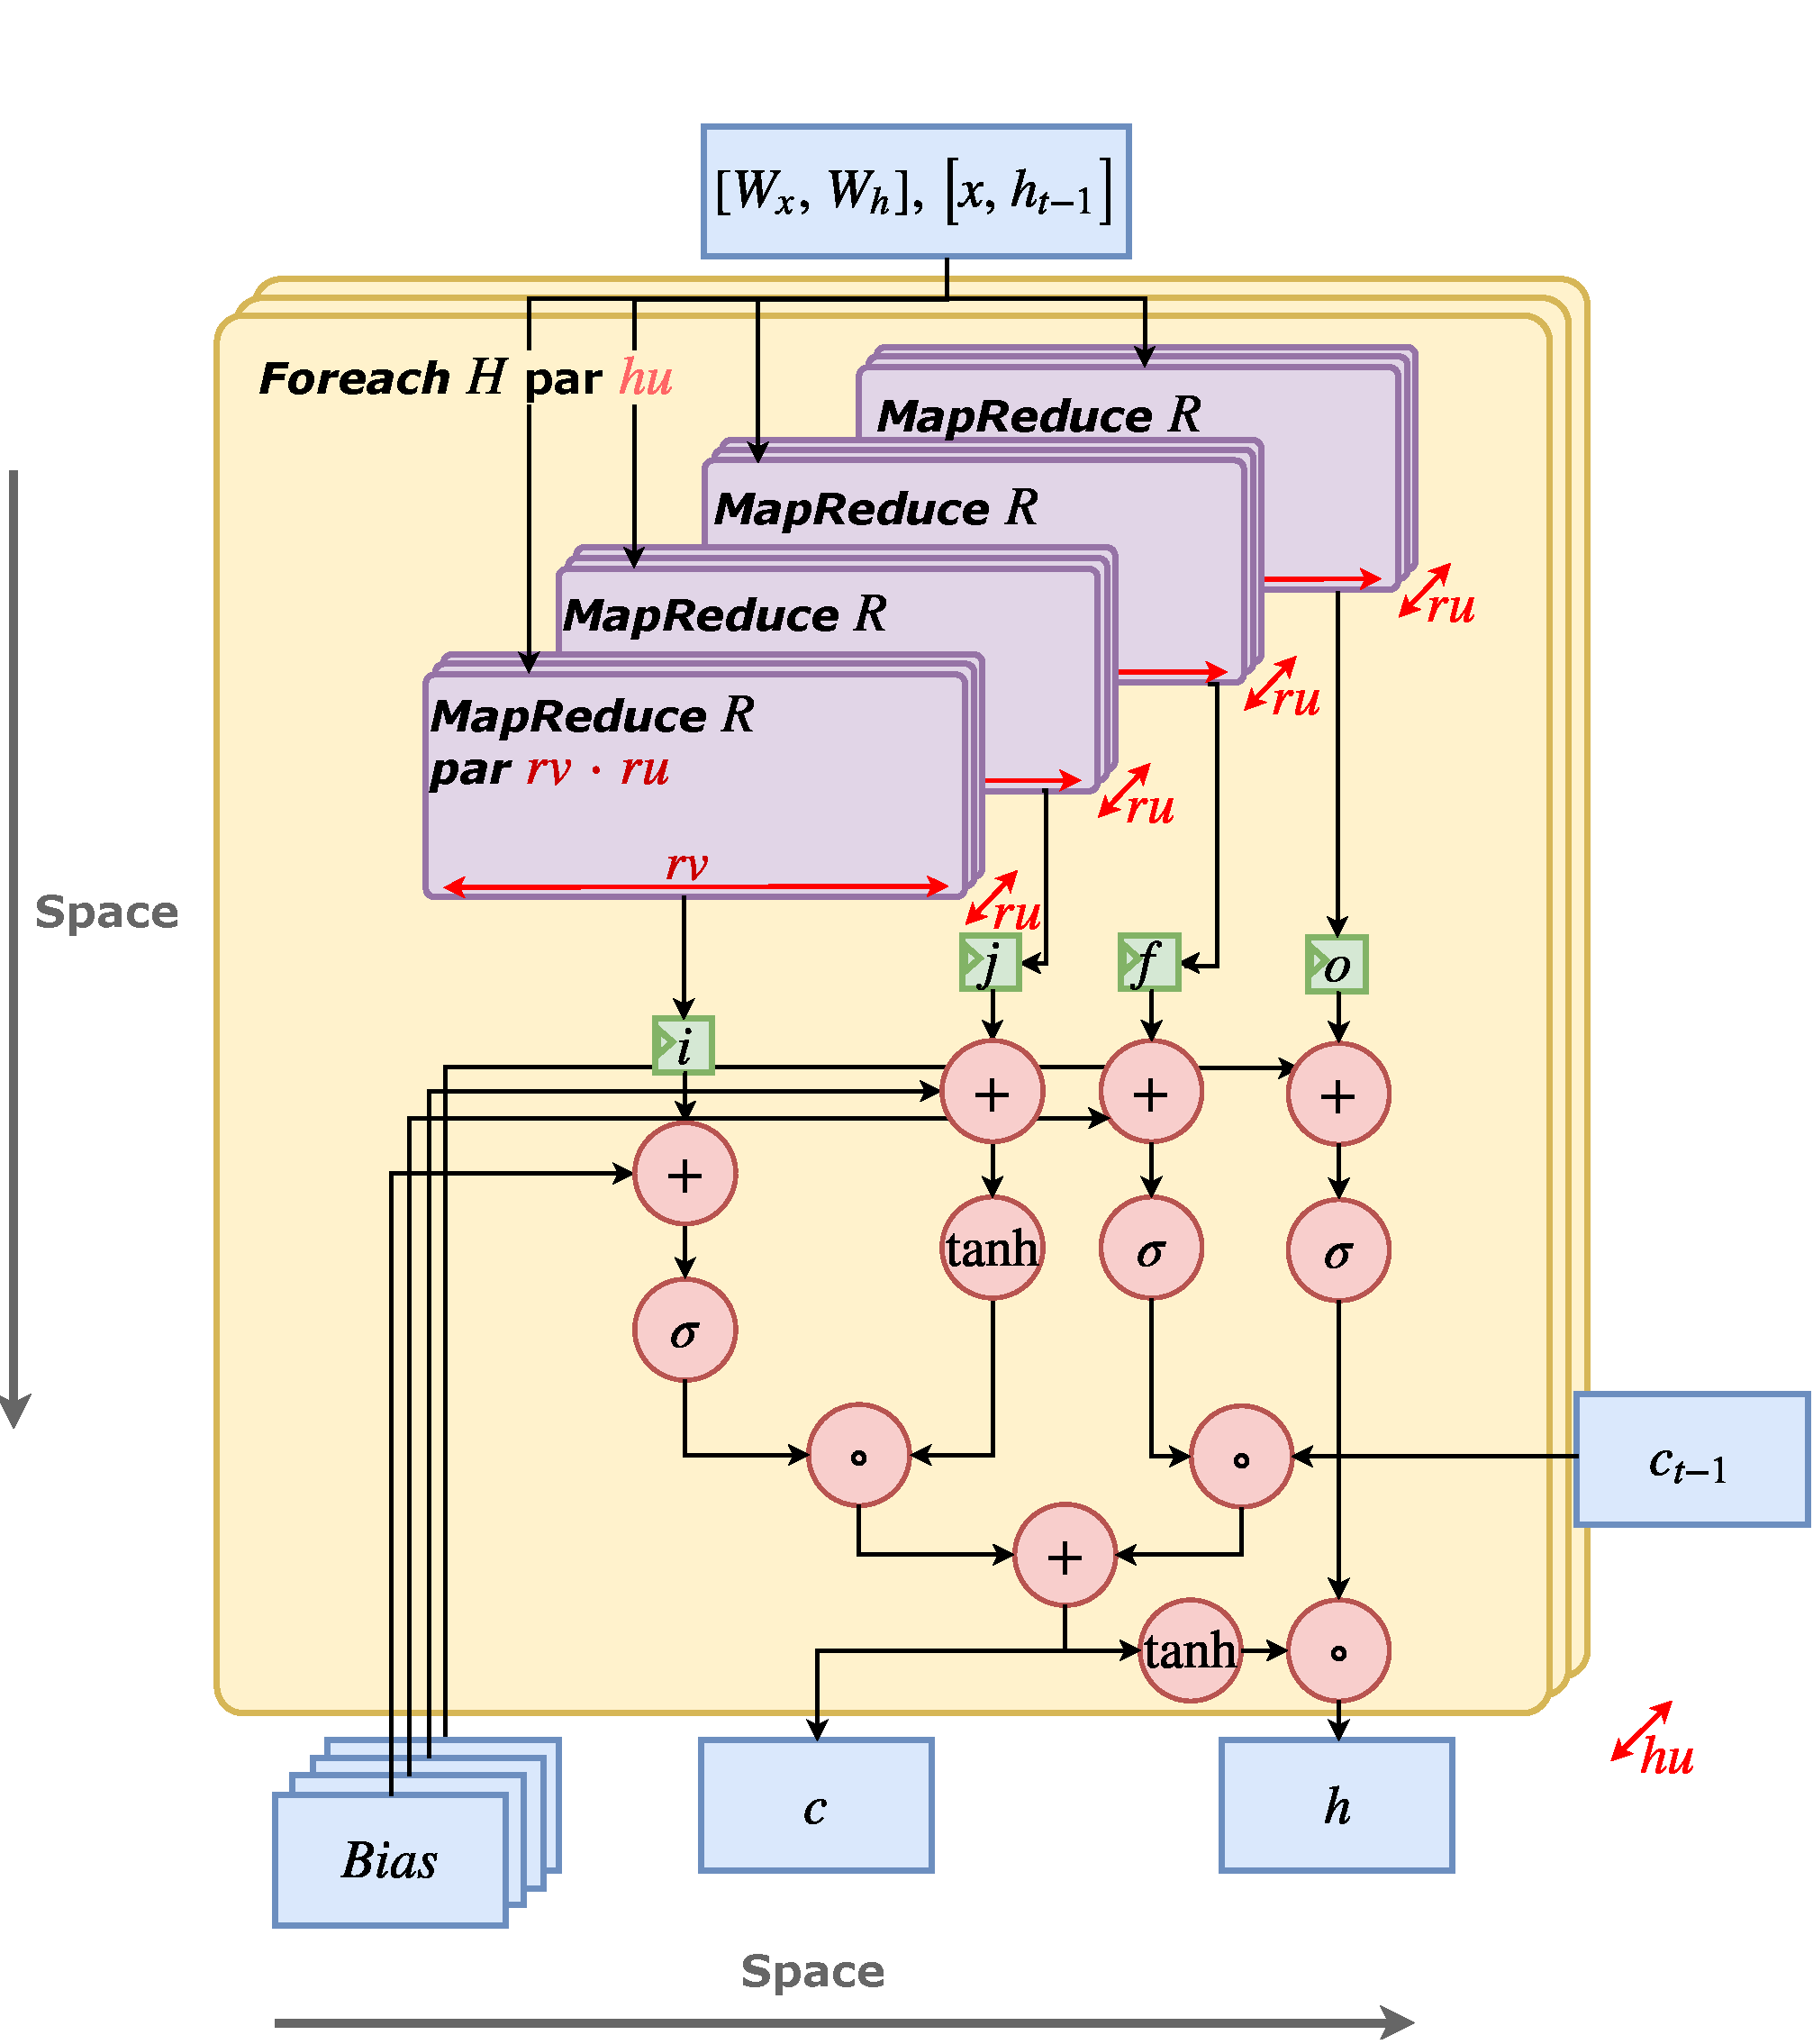
\includegraphics[width=0.9\columnwidth]{figs/splstm.pdf}
  \caption{Compute and memory layout of a loop-based LSTM design.}\label{fig:spatial_lstm}
  \vspace*{-0.2in}
\end{figure}
\begin{figure}
  \centering
  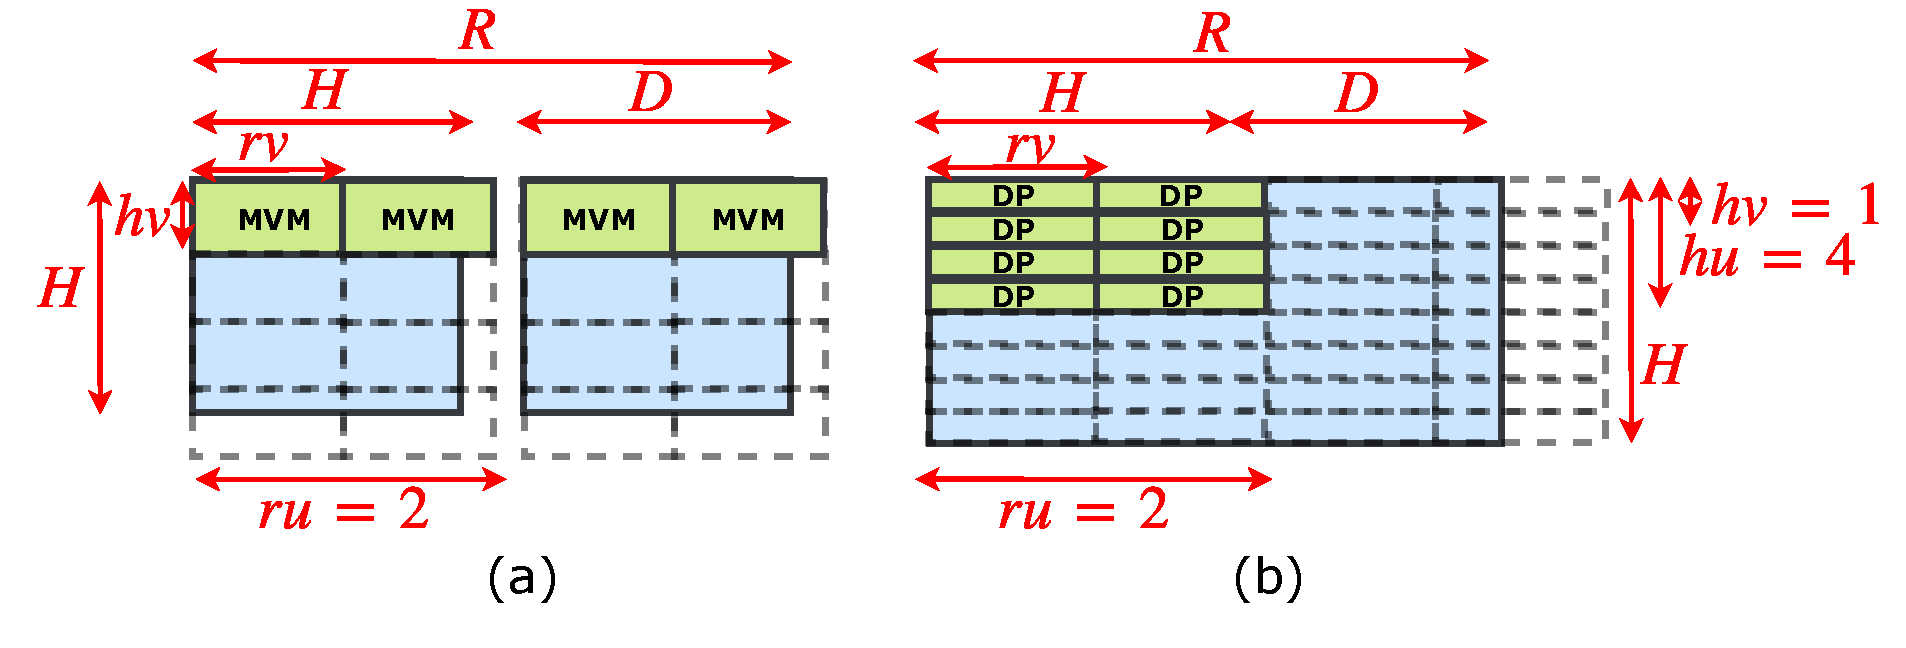
\includegraphics[width=\columnwidth]{figs/bwfrag.pdf}
   \caption{Fragmentation in an MVM-based design (a) and a loop-based design (b) in MVM.}\label{fig:bwt}
\end{figure}

As shown in Figure \ref{fig:spatial_lstm}, each MVM unit is replaced by a MapReduce unit to 
compute the tiled dot product.
Each MapReduce is vectorized by $rv$ with pipelined map function followed by a pipelined reduction tree.
$ru$ is the number of parallel MapReduce units. Results of $ru$ MapReduce blocks are reduced and 
accumulated with another reduction tree (not shown in Figure). Next, the dot product result is passed 
through a chain of function units for executing bias add and non-linear functions. Dot products, bias adds, 
and non-linear functions of the four gates can also be parallelized. Finally, the results of the four gates are pipelined
through a set of function units for element-wise operation in LSTM cell.
At the outer loop, LSTM-1 runs for $\frac{H}{hu}$ iterations,
  where $hu$ is the number of parallel LSTM-1 implementations.

In the loop-based design, all intermediate buffers are scalars as supposed to vectors. 
Regarding utilization, the loop-based LSTM design suffers from less underutilization due to unaligned problem size 
compared to the tiled MVM approach in BW. Figure \ref{fig:bwt} shows sources of such underutilizations.
An MVM approach design would suffer from 2-D fragmentation on both the $H$ and $D$ dimensions (Figure \ref{fig:bwt} (a)), whereas
the loop-based design only suffers from 1-D fragmentation on the $R$ dimension (Figure \ref{fig:bwt} (b)).

%Using BLAS terminology,
  %an LSTM-1 operation can be thought of as a new BLAS level-1 routine,
  %i.e. element-wise operations.
%In contrast, previous works mostly focus on optimizing level-2 or 3 routines.
%We find that optimizing at the lowest BLAS level allows us to utilize hardware resources more efficiently.
%In addition, using parallel patterns and loop constructs as the basic building block
  %offers sufficient abstraction and does not lead to much engineering overhead.
\begin{figure}
  \centering
  \newsavebox{\lstm}
  \begin{lrbox}{\lstm}
    \lstinputlisting[language=Spatial,linewidth=1.0\columnwidth]{code/lstm.scala}
  \end{lrbox}
  \begin{tabular} {c}
    \usebox{\lstm} \\
  \end{tabular}
  \caption{Example of LSTM in Spatial.}
\label{fig:spatial_app}
\end{figure}

Figure \ref{fig:spatial_app} shows a loop-based LSTM design implemented in Spatial.
\textbf{Foreach} is a loop construct with a lambda that takes loop iterator as input.
\textbf{Reduce} is a construct that executes MapReduce by taking a map function followed
by a reduction function. User declare explicit on-chip scratchpads and registers with
\textbf{SRAM} and \textbf{Reg}.
To enable fine-tuning an RNN application, we exposes loop vectorization factor $rv, hv$ and
unrolling factors $hu, ru$.

  \section{Plasticine Specialization for RNN Serving}
\label{sec:arch}
To show efficient execution of the loop and parallel pattern constructs,
  we map our implementation onto a spatial architecture, Plasticine.
\textbf{Foreach} at Line $17, 19$ and \textbf{Reduce} at Line $22, 23$
  are mapped to PCUs on Plasticine.
When the application size is small,
  these constructs are executed using pipelined SIMD lanes within a single PCU.
When the application size is large,
  multiple PCUs can be used to parallelize and pipeline the dot
  product across PCUs. Element-wise operations can be executed in a deep pipeline
  formed by chaining multiple PCUs.

To fit an RNN's weights on-chip,
  we execute our application with low-precision arithmetics.
In this section,
  we propose the necessary micro-architectural changes to
  support low-precision arithmetics on Plasticine.
We also discuss architectural parameter selection for Plasticine
  to serve RNN applications efficiently.

\subsection{Mixed-Precision Support}
\label{sec:arch:varprec}
Previous works \cite{fowers2018configurable, jouppi2017datacenter}
  have shown that low-precision inference can deliver promising performance
  improvements without sacrificing accuracy.
In the context of reconfigurable architectures such as FPGAs,
  low-precision inference not only increases compute density,
  but also reduces required on-chip capacity for
  storing weights and intermediate data.

To support low-precision arithmetics without sacrificing coarse-grained reconfigurability,
we introduce two low-precision struct types in Spatial: a tuple of 4 8-bit and 2 16-bit floating-point 
numbers, \texttt{4-float8} and \texttt{2-float16} respectively.
Both types packs multiple low-precision values into a single precision storage.
We support only 8 and 16-bit precisions, which are commonly seen in deep learning inference hardwares.
Users can only access values that are 32-bit aligned.
This constraint guarantees that the microarchitectual change is only local to the PCU.
Banking and DRAM access granularity remains intact from the original design.

\begin{figure}
  \centering
  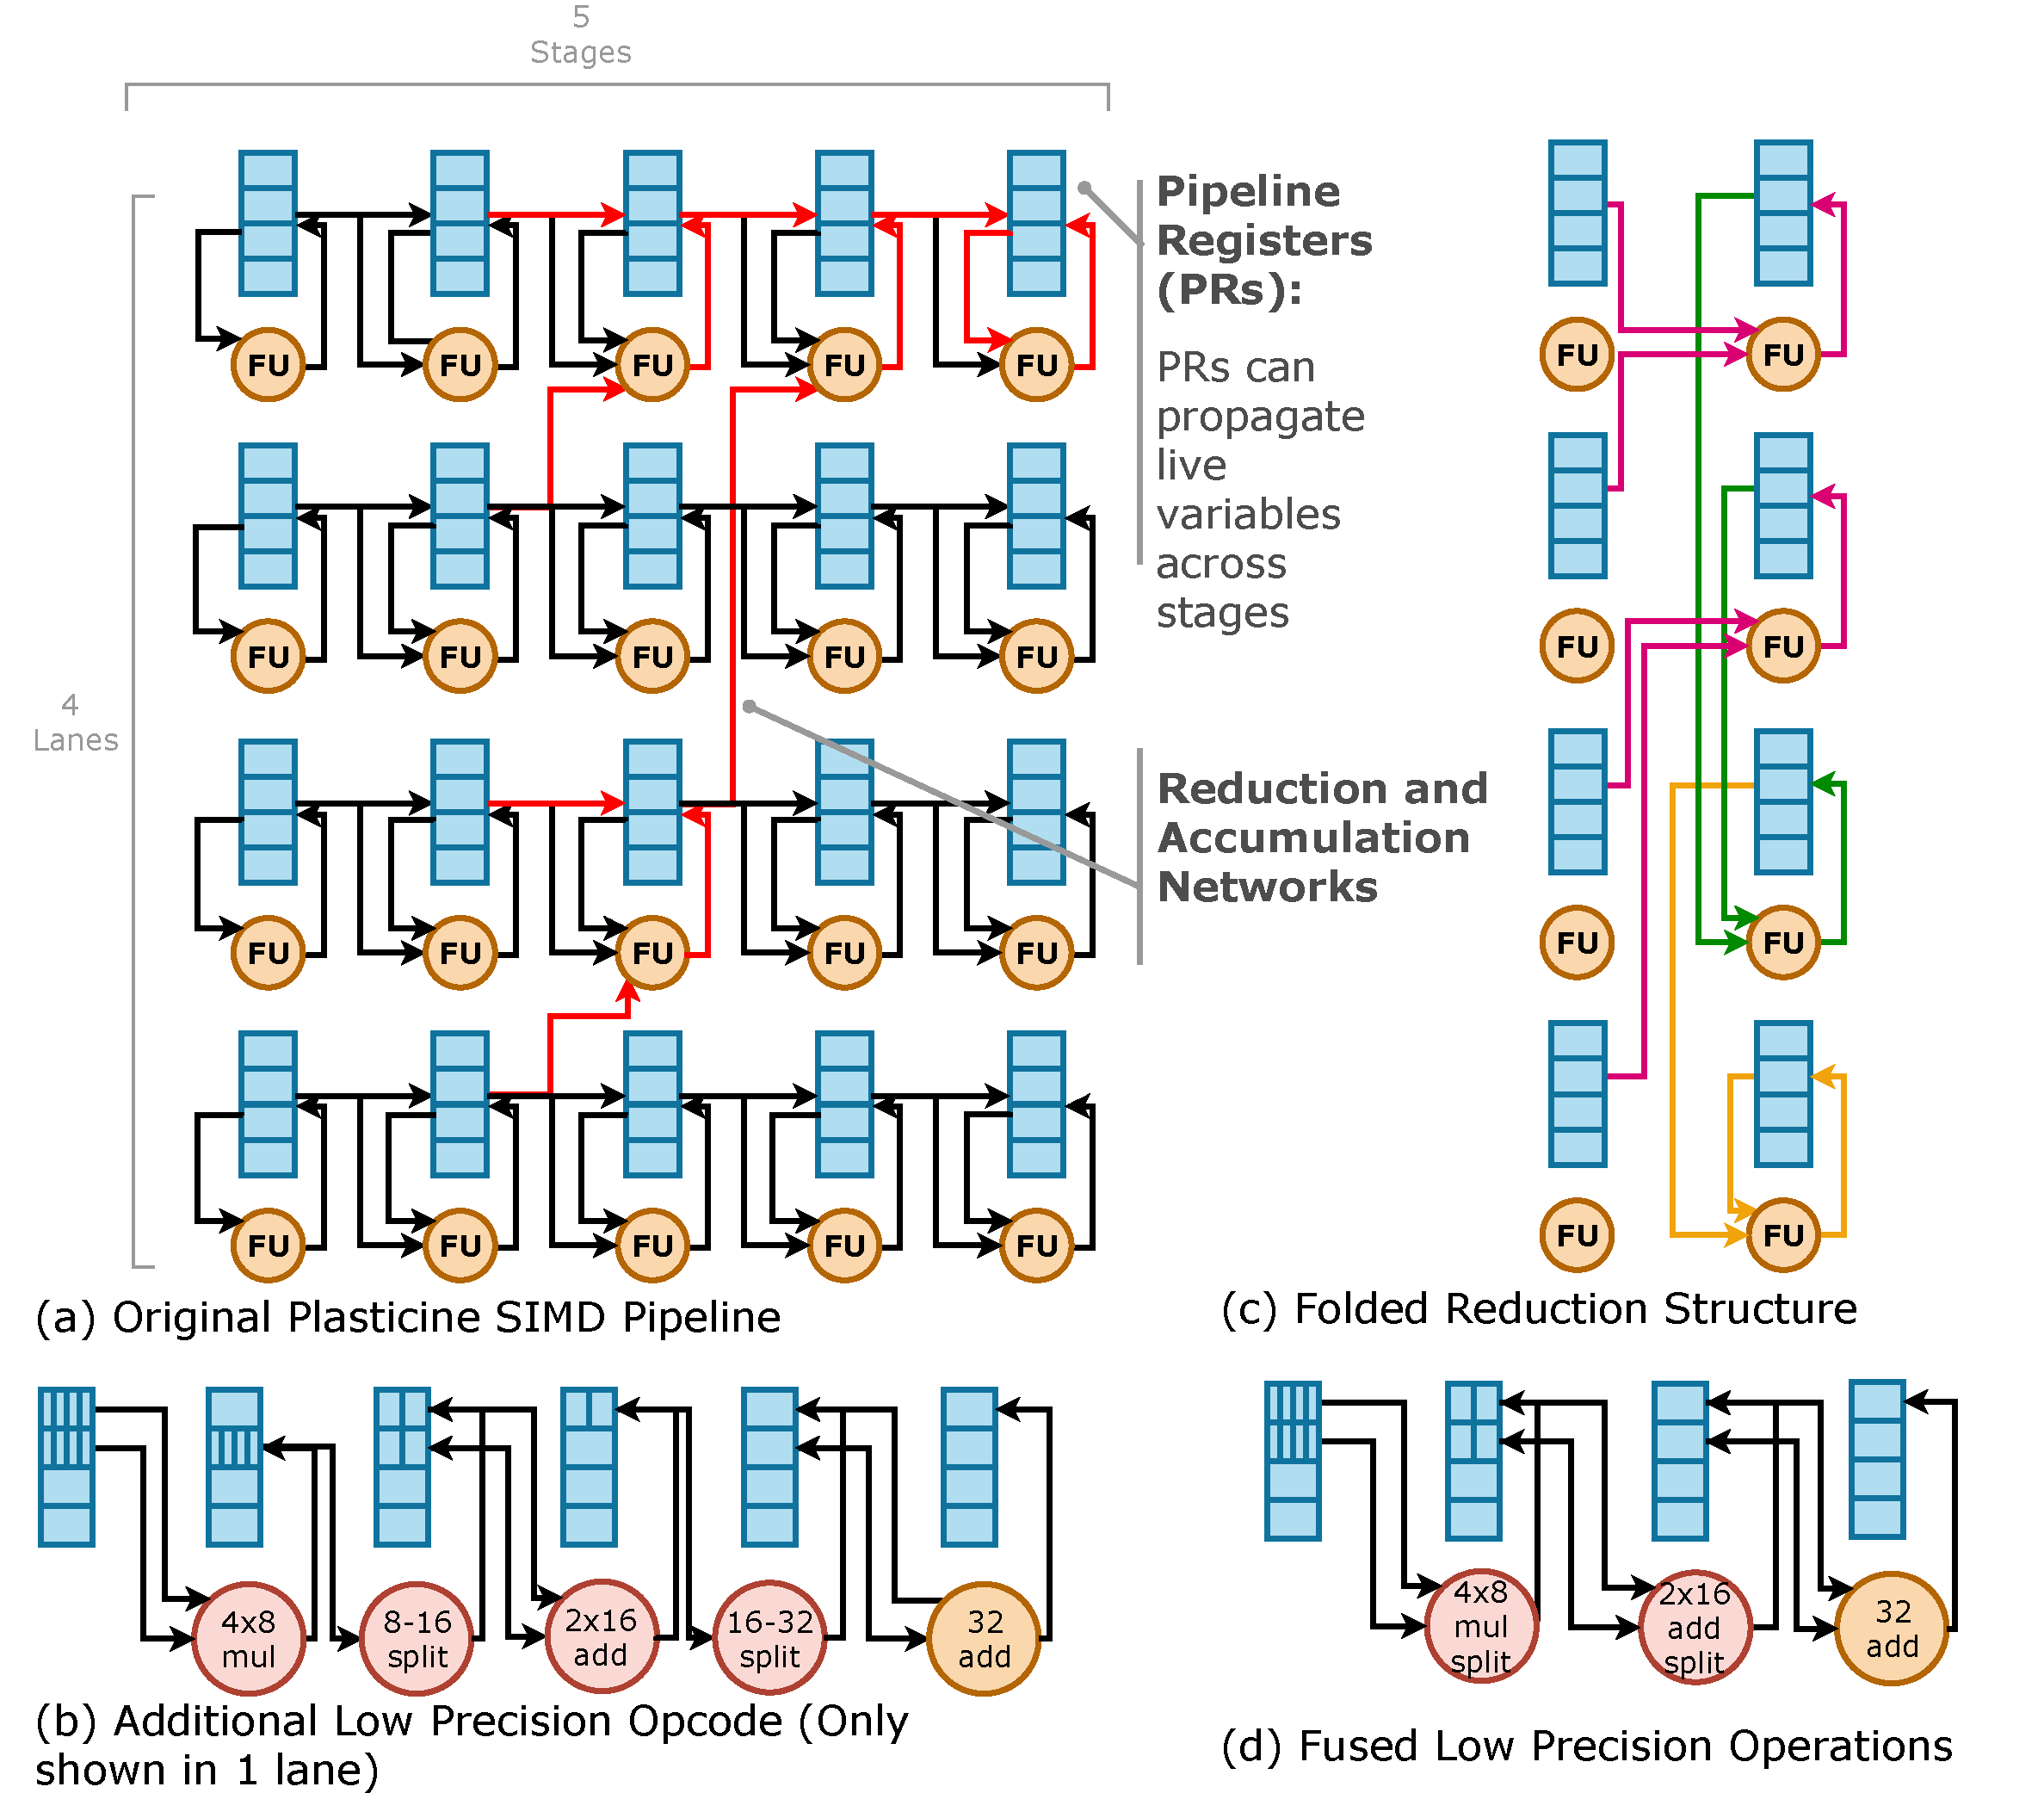
\includegraphics[width=1\columnwidth]{figs/lowprec.pdf}
  \caption{Plasticine PCU SIMD pipeline and low-precision support.
  Red circles are the new operations. Yellow circles are the original opertaions in Plasticine.
  In (d) the first stage is fused $1^{st}, 2^{nd}$ stages, and the second stage is fused
  $3^{nd}$, $4^{th}$ stages of (b).
   }
  \label{fig:lowprec}
  \vspace*{-0.3in}
\end{figure}
Figure \ref{fig:lowprec} (a) shows the original SIMD pipeline in a Plasticine PCU.
Each FU supports both floating-point and fix-point operations.
When mapping applications on Plasticine,
  the inner most loop body is vectorized across the lanes of the
SIMD pipeline, and different operations of the loop body are mapped to different stages.
Each pipeline stage contains a few pipeline registers (PRs)
  that allow propagation of live variables across stages.
%The PRs are accessible as both inputs and outputs of the FU.
%An FU can also read previous stage's PRs
%as its input value.
Special cross-lane connections as shown in red in Figure \ref{fig:lowprec} enable reduction operations.
To support 8-bit element-wise multiplication and 16-bit reduction, we add 4 opcodes to the FU, shown in
Figure \ref{fig:lowprec} (b).
The $1^{st}$ and $3^{rd}$ stages are element-wise, low-precision operations
  that multiply and add 4 8-bit and 2 16-bit values, respectively.
The $2^{nd}$ and $4^{th}$ stages rearrange low-precision values into two registers,
  and then pad them to higher precisions.
The $5^{th}$ stage reduces the two 32-bit value to a single 32-bit value using the existing add operation. 
From here, we can use the original
reduction network shown in Figure \ref{fig:lowprec} (a) to complete the remaining reduction and accumulates
in 32-bit connection.

With 4 lanes and 5 stages,
  a PCU first reads 16 8-bit values,
  performs 8-bit multiplication followed by rearrangement and padding,
  and then produce 16 16-bit values after the second stage.
The intermediate values are stored in 2 PRs per lane.
Next, 16 16-bit values are reduced to 8 16-bit values
  and then rearranged to 8 32-bit value in 2 PRs per lane.
Then, the element-wise addition in 32-bit value
  reduces the two registers in each line into 4 32-bit values.
These values are fed through the
  reduction network that completes the remaining
  reduction and accumulation in two plus one stages.

In a more aggressive specialization,
  we can fuse the multiply and rearange into the same stage.
We also fuse the first low-precision reduction with the next rearange as shown in Figure \ref{fig:lowprec} (d).
In this way, we can perform the entire low-precision map-reduce in 2 stages
  in addition to the original full precision reduction.
In order to maximize hardware reuse,
  we assume that it is possible to construct a full precision FU
  using low-precision FUs.
In addition, we observe that the original reduction network in the SIMD lanes
  could lead to low FU utilization.
To improve FU utilization, we fold the entire tree structure in a single stage.
Figure \ref{fig:lowprec} (c) shows the folded reduction accumulation structure.
Specifically, latter reductions in the tree are mapped to earlier stages in the pipeline.
In this setup, the entire reduction plus accumulation
  is still fully pipelined in $\log_2(\#_{LANE})+1$ cycles
  with no structural hazard.
With fused reduced-precision multiplication and reduction, and folded reduction tree,
  a PCU is able to perform all map-reduce that accumulates $4 \#_{LANE}$
  8-bit values using 4 stages.
All the operations are completed in $2+\log_2(\#_{LANE})+1$ cycles.

\subsection{Sizing Plasticine for Serving RNN}
Evaluating an RNN cell containing $N$ hidden units and $N$ input features
  requires $2N^2$ computations and $N^2+N$ memory reads.
With large $N$, the compute to memory ratio is 2:1.
The original Plasticine architecture uses a checkerboard layout
  with 1 to 1 ratio between PCU and PMU.
A PCU has 6 stages and 16 lanes, and a PMU has 16 banks.
This provides a 6:1 ratio between
  compute resource and on-chip memory read bandwidth.
As a result of this layout,
  on-chip memory read bandwidth becomes the bottleneck for accelerating RNN serving applications.
Given that RNNs cover a wide range of important applications,
  we select a Plasticine configuration tailored for RNN serving.
Specifically, we choose a 2 to 1 PMU-PCU ratio with 4 stages in each PCU.
Figure \ref{fig:arch} shows the layout of this Plasticine variant.
\begin{figure}
  \centering
  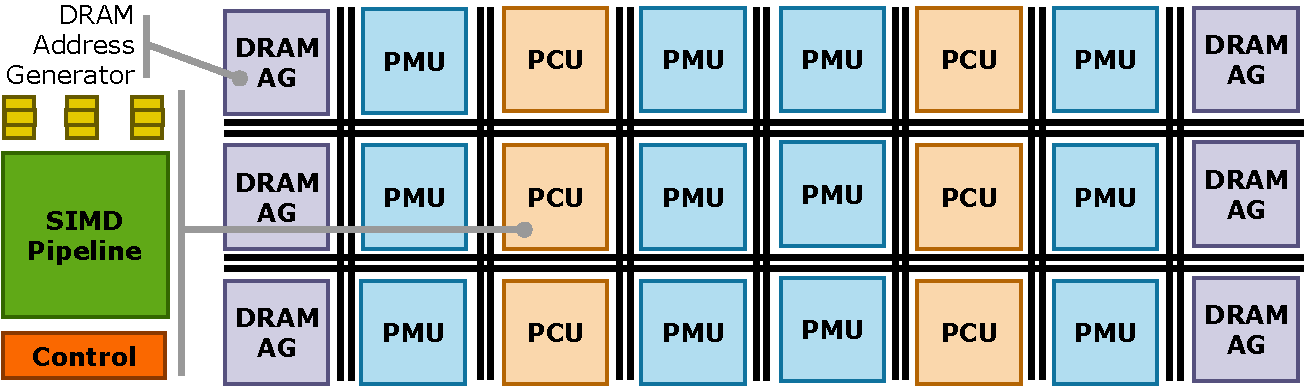
\includegraphics[width=\columnwidth]{figs/arch.pdf}
  \caption{Variant configuration of Plasticine for serving RNN.}
  \label{fig:arch}
  \vspace*{-0.2in}
\end{figure}
  \section{Evaluation} \label{sec:eval}

%% Recap work flow for readers
To evaluate our compilation flow and network architectures, we use a set of benchmarks implemented in Spatial. 
%We connect the Spatial's output IR with our low-level compiler described in section~\ref{sec:compiler}.
We start with Spatial's output IR (Section~\ref{sec:compiler}), and transform it into a graph of distributed, streaming VBs.
Our compiler then performs place and route for a target architecture before generating a configuration for cycle-accurate simulation. 
During simulation, we track the amount of data moved by each switch and router, which we integrate with synthesis results to produce estimates of area and power.

For each application, we find the highest-performing parallelization and tiling factors; for DRAM-bound applications, this is the configuration that saturates memory bandwidth.
The optimum parameters for each network configuration may vary, as high parallelization does not improve performance on a low bandwidth network.
%Next, for each optimized application, we evaluate network configurations as described in Section~\ref{sec:net_dse}.
We start with benchmark characterizations (Section~\ref{sec:app_char}), analyzing application characteristics and communication patterns to identify how they interact with networks.
Next, we characterize the area and energy of network primitives, which we use to calculate the total network area and energy in Section~\ref{sec:net_char}. 
Finally, Section~\ref{sec:network} presents a design space study over all network dimensions for both pipelined and scheduled architectures. 
Table~\ref{tab:notation} summarizes the notation we use to describe network configurations in the remainder of this section.

\subsection{Application Characterization} \label{sec:app_char}

\begin{figure}
\centering
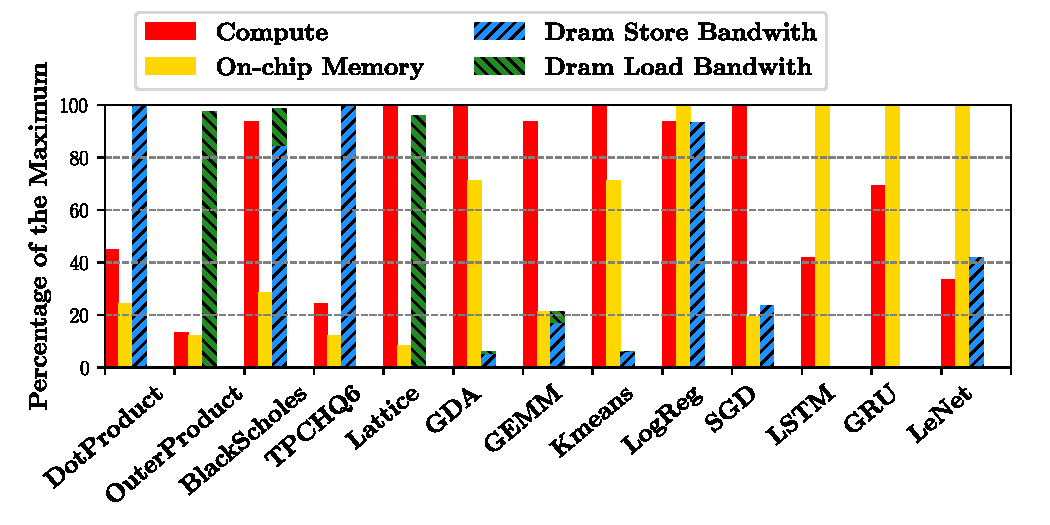
\includegraphics[width=1\columnwidth]{figs/util_bw2.pdf}
\caption{Physical resource and bandwidth utilization for various applications.}\label{fig:util_bw}
\centering
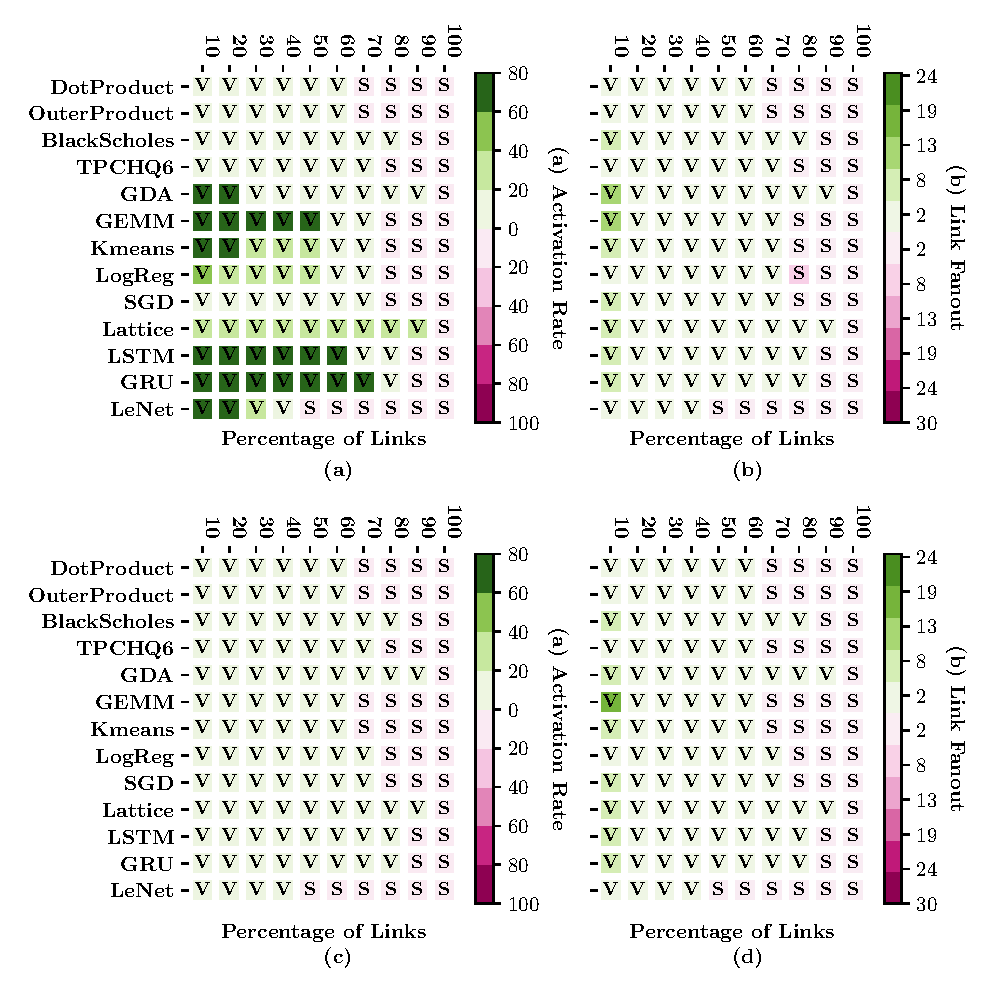
\includegraphics[width=1\columnwidth]{figs/link7.pdf}
  \caption{Application communication patterns on pipelined (a,b) and scheduled (c,d) CGRA architectures.
  (a) and (c) show the activation rate distribution of logical links at runtime. 
  Links sorted by granularity, then rate; darker boxes indicate higher rates.
  The split between green and pink shows the ratio of logical vector to scalar links. (b) and (d) show the distribution of broadcast link fanouts.
 }\label{fig:link}
\end{figure}

\begin{figure}
\centering
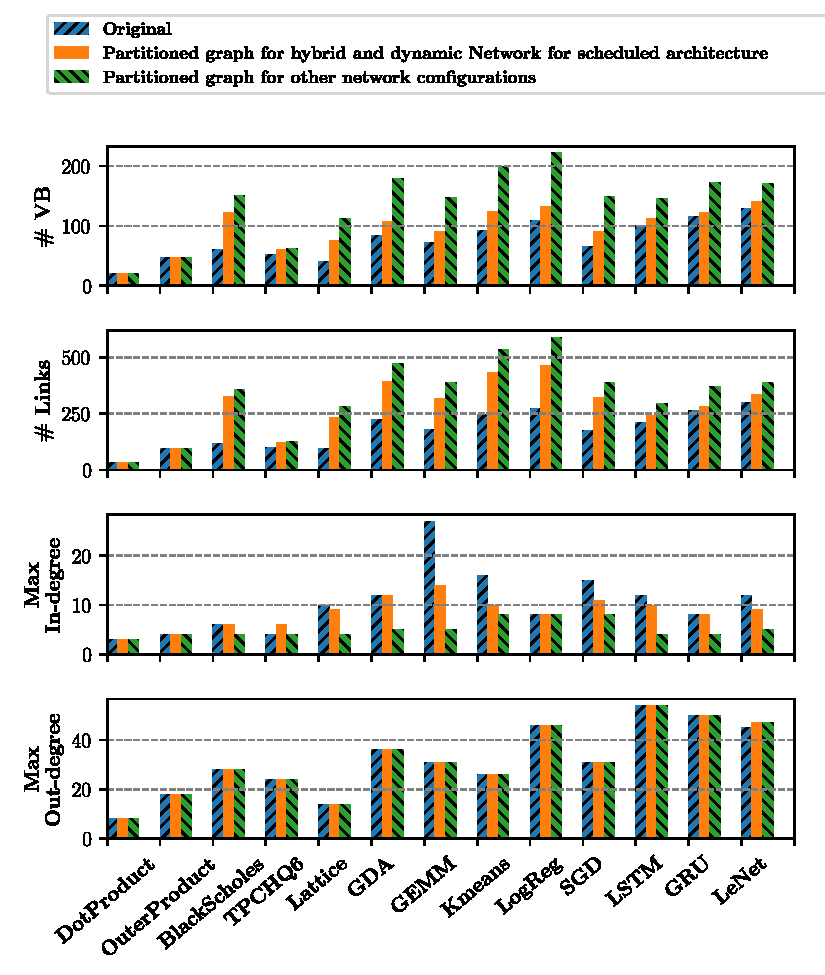
\includegraphics[width=1\columnwidth]{figs/graph.pdf}
\caption{Characteristics of program graphs.}\label{fig:graph}
\end{figure}

We select a mix of applications from domains where hardware accelerators have shown promising performance and energy-efficiency benefits, such as linear algebra, databases, and machine learning.
Table~\ref{tab:benchmark} lists the applications and their data size.
Figure~\ref{fig:util_bw} shows, for each design, which resource limits performance: compute, on-chip memory, or DRAM bandwidth. 
%Variations in these application characteristics introduce different on-chip network requirements.
DotProduct, TPCHQ6, OuterProduct, and BlackScholes are DRAM bandwidth-bound applications. 
These applications use few on-chip resources to achieve maximum performance, resulting in minimal communication.
Lattice (a fast inference model for low-dimensional regression~\cite{garcia2009lattice}), GDA, Kmeans, SGD, and LogReg are compute-intensive applications; for these, maximum performance requires using as much parallelization as possible. 
Finally, LSTM, GRU, and LeNet are applications that are limited by on-chip memory bandwidth or capacity. 
For compute- and memory-intensive applications, high utilization translates to a large interconnection network bandwidth requirement to sustain application throughput. 

Figure~\ref{fig:link}(a,b) shows the communication pattern of applications
characterized on the pipelined CGRA architecture, including the variation in communication granularity. 
Compute and on-chip memory-bound applications show a significant amount of high-bandwidth communication (links with almost 100\% activity). 
A few of these high-bandwidth links also exhibit high broadcast fanout. 
Therefore, a network architecture must provide sufficient bandwidth and efficient broadcasts to sustain program throughput.
On the contrary, time-scheduled architectures, shown in Figure~\ref{fig:link}(c,d), exhibit
lower bandwidth requirements due to the lower throughput of individual compute PBs. 
Even applications limited by on-chip resources have less than a 30\% firing rate on the busiest logical links; this reveals an opportunity for link sharing without sacrificing performance.

Figure~\ref{fig:graph} shows statistics describing the VB dataflow graph before and after partitioning.
The blue bars show the number of VBs, number of logical links, and maximum VB input/output degrees in the original parallelized program; the yellow and green bars show the same statistics after partitioning. 
Fewer VBs are partitioned for hybrid networks and dynamic networks with the time-scheduled architecture, as explained in Section~\ref{sec:partition}. 
The output degree does not change with partitioning because most outputs with a large degree are from broadcast links.

\subsection{Area and Energy Characterization} \label{sec:net_char}

Figure~\ref{fig:sweep} shows that switch and router power scale linearly with the rate of data transmission, but that there is non-zero power at zero-load. 
For simulation, the duty cycle refers to the amount of offered traffic, not accepted traffic.
Because our router uses a crossbar without speedup \cite{dallytowles}, the testbench saturates the router at 60\% duty cycle when providing uniform random traffic. 
Nonetheless, router power still scales linearly with accepted traffic.

A sweep of different switch and router parameters is shown in Figure~\ref{fig:char}. Subplots (d,e,f) show the energy necessary to transmit a single bit through a switch or router.
Subplot (a) shows the roughly quadratic scaling of switch area with the number of links between adjacent switches.
Vector switches scale worse with increasing bandwidth than scalar switches, mostly due to increased crossbar wire load. 
At the same granularity, a router consumes more energy a switch to transmit a single bit of data, even though the overall router consumes less power (as shown in Figure~\ref{fig:sweep}); 
this is because the switch has a higher throughput than the router.
The vector router has lower per-bit energy relative to the scalar router because it can amortize the cost of allocation logic, whereas the vector switch has higher per-bit energy relative to the scalar switch due to increased capacitance in the large crossbar. 
Increasing the number of VCs or buffer depth per VC also significantly increases router area and energy, but reducing the router flit width can significantly reduce router area. 

Overall, these results show that scaling static bandwidth is cheaper than scaling dynamic bandwidth, and a dynamic network with small routers can be used to improve link sharing for low bandwidth communication.  
We also see that a specialized scalar network, built with switches, adds negligible area compared to and is more energy efficient than the vector network. 
Therefore, we use a static scalar network with a bandwidth of 4 for the remainder of our evaluation, except when evaluating the pure dynamic network.
The dynamic network is also optimized for the rare instances when the static scalar network is insufficient. 
When routers transmit scalar data, the high bits of data buffers are clock-gated, reducing energy as shown in (f).
Figure~\ref{fig:area} summarizes the area breakdown of all the network configurations that we evaluate.
\subsection{Network Architecture Exploration} \label{sec:net_dse}

\begin{table}
\footnotesize
\begin{tabular*}{\columnwidth}{p{1cm} p{7cm}}
  \bottomrule
  \textbf{Notation} & \textbf{Description} \\\midrule
  $[$S,H,D$]$ & Static, hybrid, and dynamic network \\\midrule
  x\# & Static bandwidth on vector network (\#links between switches) \\\midrule
  %$s\#$ & Number of links between switches on static scalar network \\\midrule
  f\# & Flit width of a router or vector width of a switch \\\midrule
  v\# & Number of VC in router \\\midrule
  b\# & Number of buffers per VC in router \\\midrule
  $[$db,cd$]$ & Buffered vs. credit-based flow control in switch \\\midrule
  %$[Scheduled, Pipelined]$ & Time scheduled vs deep pipelined accelerator architectures \\\midrule
\end{tabular*}
\caption{Network design parameter summary.}
\label{tab:notation}
\end{table}
\begin{figure}
\centering
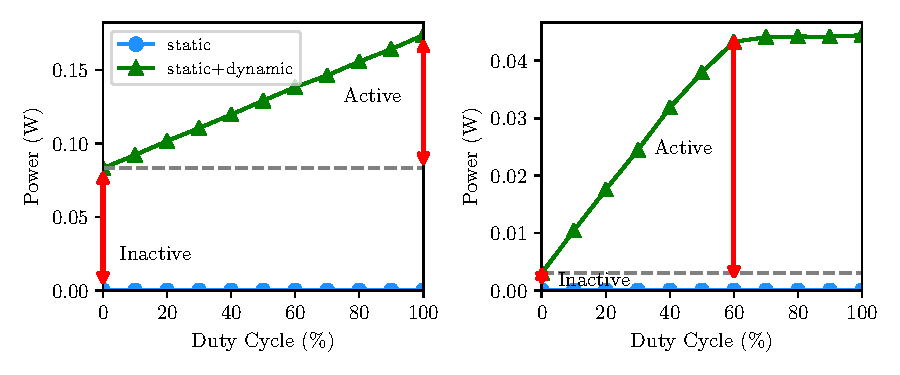
\includegraphics[width=1\columnwidth]{figs/sweep.pdf}
  \caption{Switch and router power with varying duty cycle.}\label{fig:sweep}
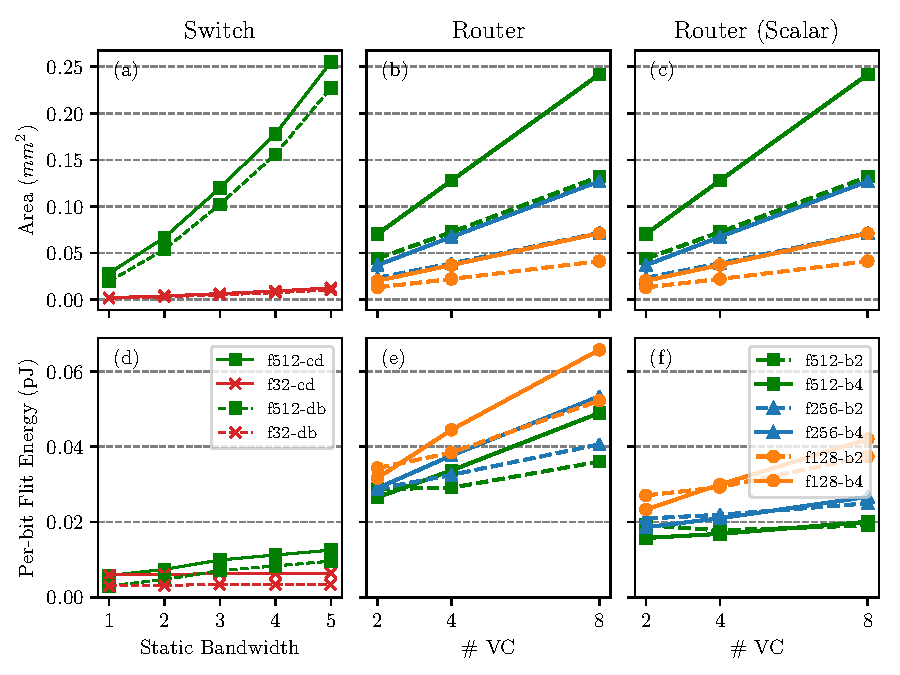
\includegraphics[width=1\columnwidth]{figs/char.pdf}
  \caption{Area and per-bit energy for (a,d) switches and (b,c,e,f) routers. 
  (c,f) Subplots (c,f) show area and energy of the vector router when used for scalar values (32-bit).}\label{fig:char}
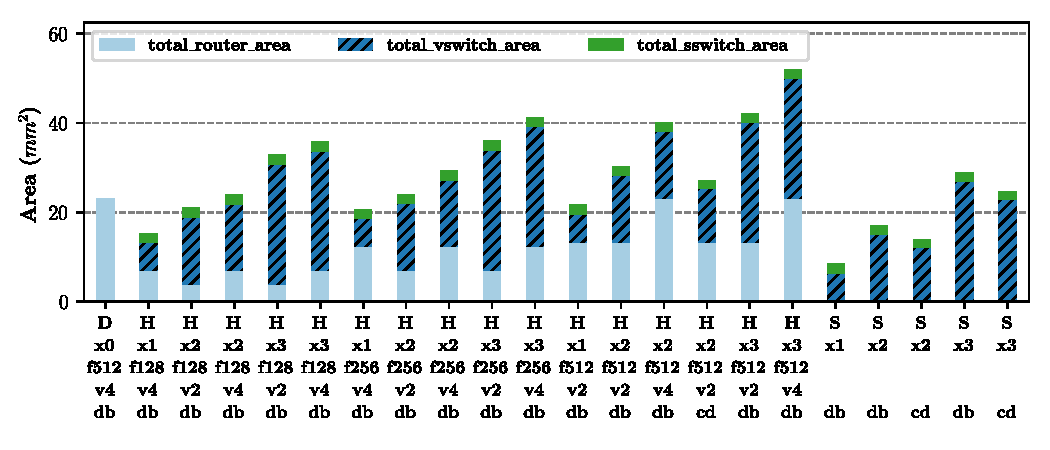
\includegraphics[width=1\columnwidth]{figs/area.pdf}
  \caption{Area breakdown for all network configurations.}\label{fig:area}
\end{figure}

We evaluate our network configurations in five dimensions: performance (perf), performance per network area (perf/area), performance per network
power (perf/watt), network area efficiency (1/area), and network power efficiency (1/power). 
Among these metrics, performance is the most important: networks only consume a small fraction of the overall accelerator area and energy (roughly 10-20\%). 
Because the two key advantages of hardware accelerators are high throughput and low latency, 
we filter out a network design point if it introduces
more than 10\% performance overhead.
This is calculated by comparing to an ideal network with infinite bandwidth and zero latency.

For metrics that are calculated per application, such as performance, performance/watt, and power efficiency, we first normalize the metric with respect to the 
worst network configuration for that application. 
For each network configuration, we present a geometric mean normalized across all applications. 
For all of our experiments, except Section~\ref{sec:scale}, we use a network
size of $14\times14$ end-point PBs. All vector networks use a vectorization factor of 16 (\SI{512}{bit} messages).

\begin{figure}
\centering
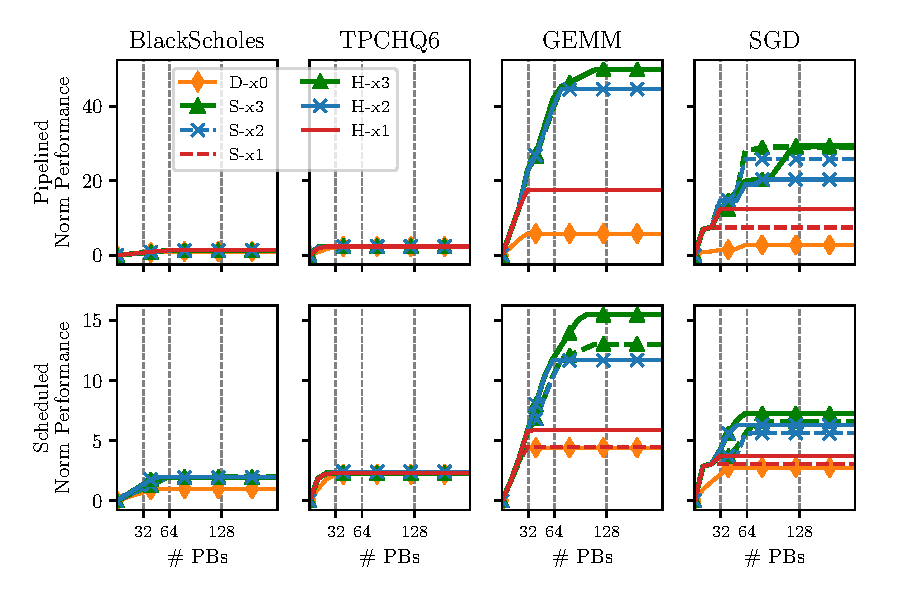
\includegraphics[width=1\columnwidth]{figs/scale.pdf}
\caption{Performance scaling with increased CGRA grid size for different networks.}\label{fig:scale}
\end{figure}
\subsubsection{Bandwidth scaling with network size}\label{sec:scale}
%Figure~\ref{fig:scale} shows the performance scaling of applications as accelerator size scales with different network configurations.
Figure~\ref{fig:scale} shows how different networks allow several applications to scale to different numbers of PBs.
For IO-bound applications (BlackScholes and TPCHQ6), performance does not scale with additional compute and on-chip memory resources.
However, the performance of compute-bound applications (GEMM and SGD) improves with increased resources, but plateaus at a level that is determined by on-chip network bandwidth. 
%Although this is expected for general network designs, it is much more noticeable due to the high-bandwidth communication inherent in pipelined reconfigurable accelerators.
This creates a trade-off in accelerator design between highly vectorized compute PBs with a small network---which would be underutilized for non-vectorized problems---and smaller compute PBs with limited performance due to network overhead. 
For more finely grained compute PBs, both more switches and more costly (higher-radix) switches must be employed to meet application requirements.

The scaling of time-scheduled accelerators (bottom row) is much less dramatic than that of deeply pipelined architectures (top row). 
Although communication between PBs in these architectures is less frequent, the scheduled architecture must use additional parallelization to match the throughput of the pipelined architecture; this translates to larger network sizes. 
%Since scaling dynamic bandwidth is much more expensive than scaling static bandwidth, as shown in section \ref{sec:net_char}, 
%we only explored scaling bandwidth in vector switches. 

For pipelined architectures, both hybrid and static networks provide similar scaling with the same static bandwidth:
the additional bandwidth from the dynamic network in hybrid networks does not provide additional scaling. 
This is mostly due to a bandwidth bottleneck between a PB and its router, which prevents the PB from requesting multiple elements per cycle.
Hybrid networks tend to provide better scaling for time-scheduled architectures; multiple streams can be time multiplexed at each ejection port without losing performance.

\begin{figure}
\centering
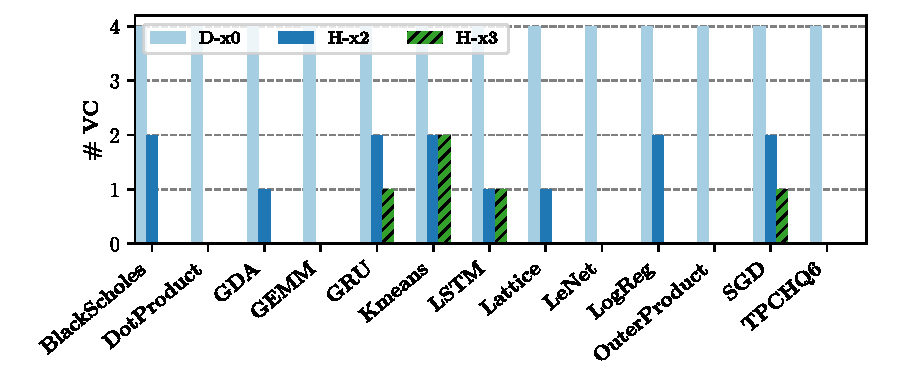
\includegraphics[width=1\columnwidth]{figs/vc.pdf}
  \caption{Number of VCs required for dynamic and hybrid networks. (No VCs indicates that all traffic is mapped to the static network.)}\label{fig:vc}
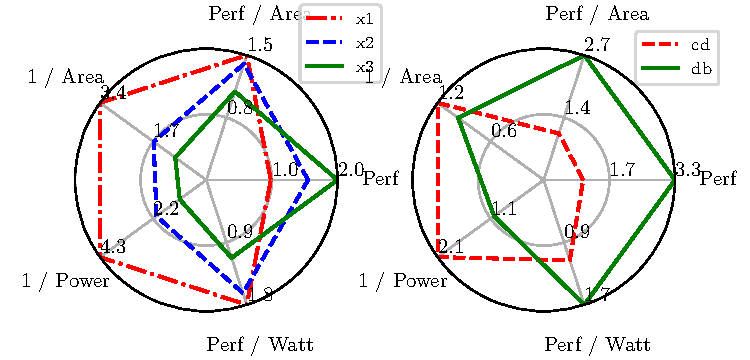
\includegraphics[width=1\columnwidth]{figs/radar_switch.pdf}
  \caption{
    Impact of bandwidth and flow control strategies in switches.}\label{fig:radar_switch}
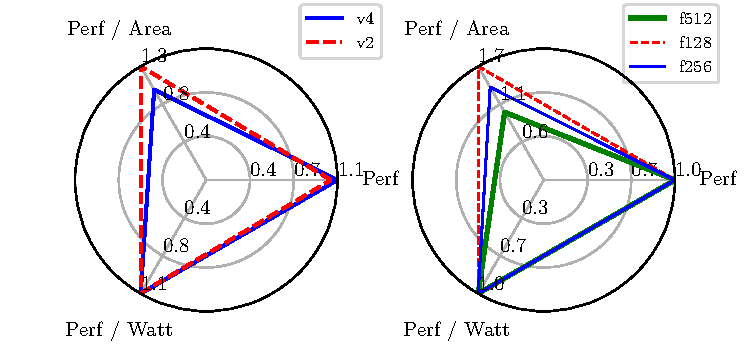
\includegraphics[width=1\columnwidth]{figs/radar_router.pdf}
  \caption{Impact of VC count and flit widths in routers.}\label{fig:radar_router}
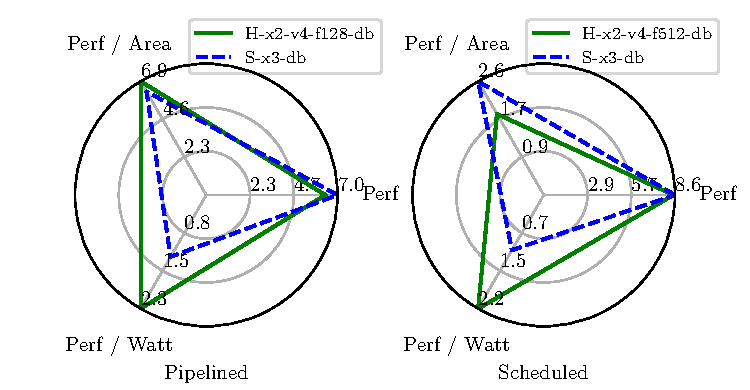
\includegraphics[width=1\columnwidth]{figs/radar_best.pdf}
  \caption{Geometric mean improvement for the best network configurations, relative to the worst configuration.}\label{fig:radar_best}
\end{figure}

\begin{figure*}
\centering
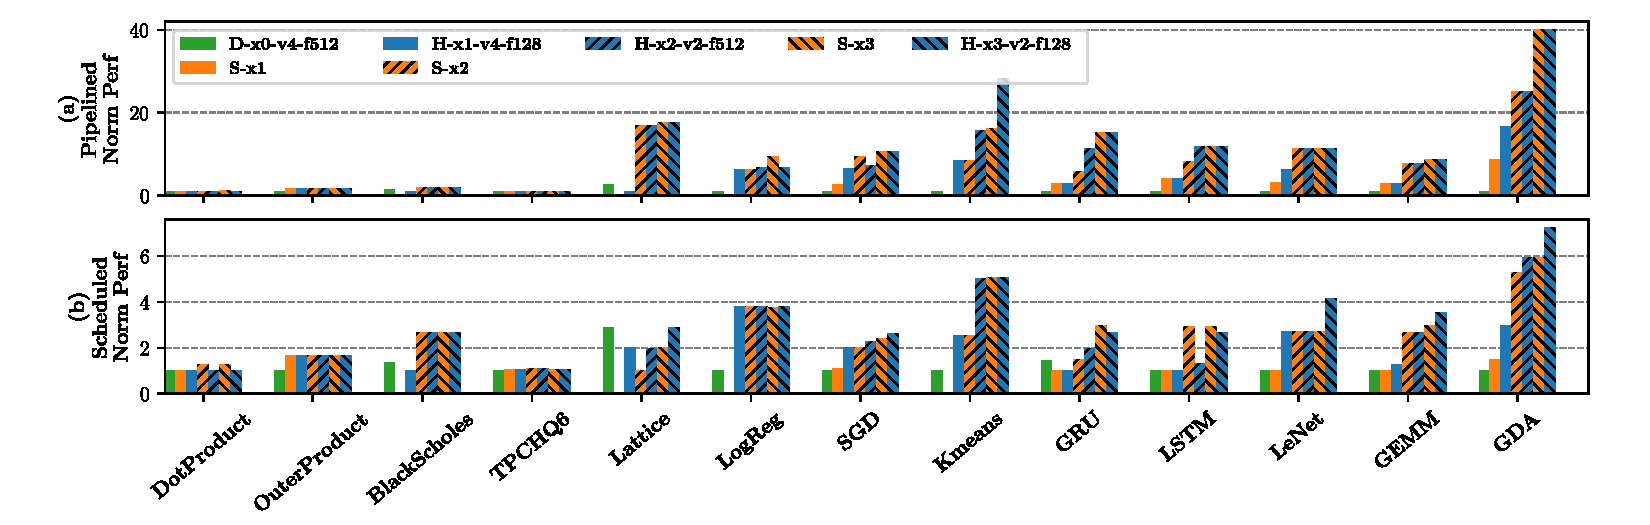
\includegraphics[width=1\linewidth]{figs/perf.pdf}
  \caption{Normalized performance for different network configurations.}\label{fig:perf}
\end{figure*}

\begin{figure}
\centering
  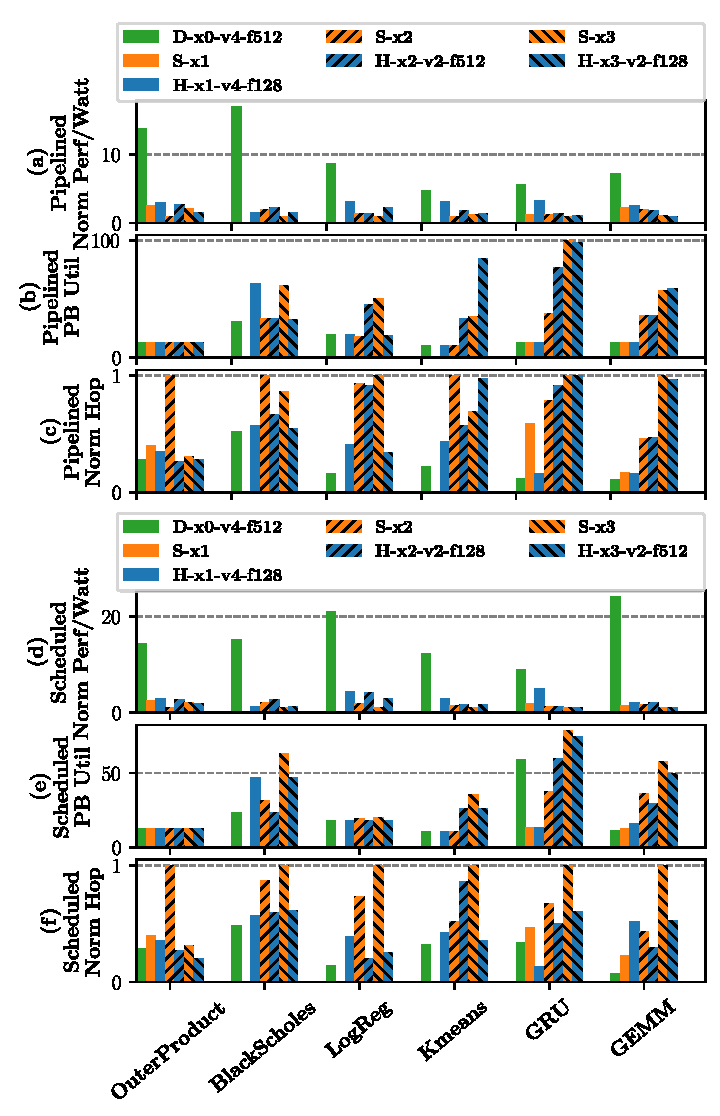
\includegraphics[width=1\columnwidth]{figs/energy.pdf} 
\caption{(a,d): Normalized performance/watt. (b,e): Percentage of compute and memory PBs utilized for each network configuration. 
  (c,f): Total data movement (hop count).}
\label{fig:energy}
\end{figure}

\subsubsection{Bandwidth and flow control in switches}

In this section, we study the impact of static network bandwidth and flow control mechanism (per-hop vs. end-to-end credit-based). 
On the left side of Figure~\ref{fig:radar_switch}, we show that increased static bandwidth results in a linear performance increase and a superlinear increase in area and power. 
As shown in Section~\ref{sec:scale}, any increase in accelerator size must be coupled with increased network bandwidth to effectively scale performance. 
This indicates that network overhead will increase with the size of an accelerator.

The right side of Figure~\ref{fig:radar_switch} shows that, although credit-based flow control reduces the amount of buffering in switches and decreases network area and energy, application performance is significantly impacted. 
This is the result of imbalanced data-flow pipelines in the program: when there are parallel long and short paths over the network, there must be sufficient buffer space on the short path equal to the product of throughput and the difference in latency. 
Because performance is our most important metric, credit-based flow control is not feasible, especially because the impact of bubbles increases with communication distance, and therefore network size.

\subsubsection{VC count and reduced flit width in routers}
In this experiment, we study the area-energy-performance trade-off between routers with different VC counts. As shown
in Section~\ref{sec:net_char}, using many VCs increases both network area and energy.
However, using too few VCs may force roundabout routing on the dynamic network or result in VC allocation failure when the network is heavily utilized.
Nonetheless, the left side of Figure~\ref{fig:radar_router} shows minimal performance improvement from using more VCs. 

Therefore, for each network design, we use a VC count equal to the maximum number of VCs required to map all applications to that network. 
Figure~\ref{fig:vc} shows that the best hybrid network configurations with 2x and 3x static bandwidth require at most 2 VCs, whereas the pure dynamic network requires 4 VCs to map all applications.
%This is different from a traditional processor based (request-response) architecture because, first, less VCs are required to map a large amount of traffic onto dynamic network due deadlock challenges
%specific to streaming architectures, second, communication is much infrequent to incur bandwidth penalty on dynamic network. 
Because dynamic network communication is infrequent, hybrid networks with fewer VCs provide both better energy and area efficiency than networks with more VCs, even though this constrains routing on the dynamic network.
%The improvement is less significant in a time-scheduled architecture because of an overall reduction in required bandwidth.

We also explore the effects of reducing dynamic network bandwidth by using smaller routers;
as shown in Section~\ref{sec:net_char}, routers with smaller flits have a much smaller area.
Ideally, we could scale static network bandwidth while using a low-bandwidth router to provide an escape path and reduce overall area and energy overhead. 
The right side of Figure~\ref{fig:radar_router} shows that, for a hybrid network, reducing flit width improves area efficiency with minimal performance loss. 

%The reduction in performance is more significant in pipelined CGRAs than time-scheduled CGRAs, as the latter has a lower bandwidth requirement.

\subsubsection{Static vs. hybrid vs. dynamic networks}

Figure~\ref{fig:perf} shows the normalized performance for each application running on several network configurations.
%For some applications, the ideal configuration could not be placed and routed onto a static network with 1x bandwidth; missing bars for S-x1 are the result of these failures.
For some applications, the bar for S-x1 is missing; this indicates that place and route failed for all unrolling factors.
For DRAM-bound applications, the performance variation between different networks is trivial because only a small fraction of the network is being used. 
In a few cases (Kmeans and GDA), hybrid networks  provide better performance due to slightly increased bandwidth.
For compute-bound applications, performance primarily correlates with network bandwidth because more bandwidth permits a higher parallelization factor. 

%Figures~\ref{fig:energy} [1,4] show the normalized performance/watt of the network for pipelined and scheduled
%architectures. Figure [2,5] show the corresponding PB utilizations in the network. Figure [3,6] summarize the total
%data movement distributed on static vector, static scalar, dynamic vector and dynamic scalar for that network
%configuration.  
The highest bandwidth static network uses the most PBs, as shown in Figures~\ref{fig:energy}(b,e), because it permits more parallelization. 
It also has more data movement, as shown in (c,f), because PBs can be distributed farther apart. 
Due to bandwidth limitations, low-bandwidth networks perform best with small unrolling factors---they are unable to support the bisection bandwidth of larger program graphs.
This is evident in Figures~\ref{fig:energy}(b,e), where networks D-x0-v4-f512 and S-x2 have small PB utilizations.

With the same static bandwidth, most hybrid networks have better energy efficiency than the corresponding pure static networks, even though routers take more energy than switches to transmit the same amount of data.
This is a result of allowing a small amount of traffic to escape onto the dynamic network: with the dynamic network as a safety net, static place and route tends to converge to better placements with less overall communication.
This can be seen in Figures~\ref{fig:energy}(c,f), where most static networks have larger hop counts than the corresponding hybrid network; hop count is the sum of all runtime link traversals, normalized per-application to the network configuration with the most hops.
Subplots (e,f) show that more PBs are utilized with static networks than hybrid networks.
%Compared to hybrid networks, (e,f), show larger PB utilization at the same parallelization factor on the purely static network .
This is because the compiler imposes less stringent IO constraints on PBs when partitioning for the hybrid network (as explained in Section~\ref{sec:partition}), which results in fewer PBs, less data movement, and greater energy efficiency for hybrid networks.

In Figure~\ref{fig:radar_best}, we summarize the best perf/watt and perf/area (among network configurations with <10\% performance overhead) for pipelined and scheduled CGRA architectures. 
Pure dynamic networks are not shown because they perform poorly due to insufficient bandwidth.
On the pipelined CGRA, the best hybrid network provides a 6.4x performance increase, 2.3x better energy efficiency, and a 6.9x perf/area increase over the worst network configuration. 
The best static network provides 7x better performance, 1.2x better energy efficiency, and 6.3x better perf/area. 
The hybrid network gives the best perf/area and perf/watt, with a small degradation in performance when compared to the static network. 
On the time-scheduled CGRA, both static and hybrid networks have an 8.6x performance improvement. 
The hybrid network gives a higher perf/watt improvement at 2.2x, whereas the static network gives a higher perf/area improvement at 2.6x.
Overall, the hybrid networks deliver better energy efficiency with shorter routing distances by allowing an escape path on the dynamic network.

%It can also provide a decent area efficiency when coupled with a small dynamic network with a minimum performance penalty. 

%\begin{figure}[ht]
%\centering
%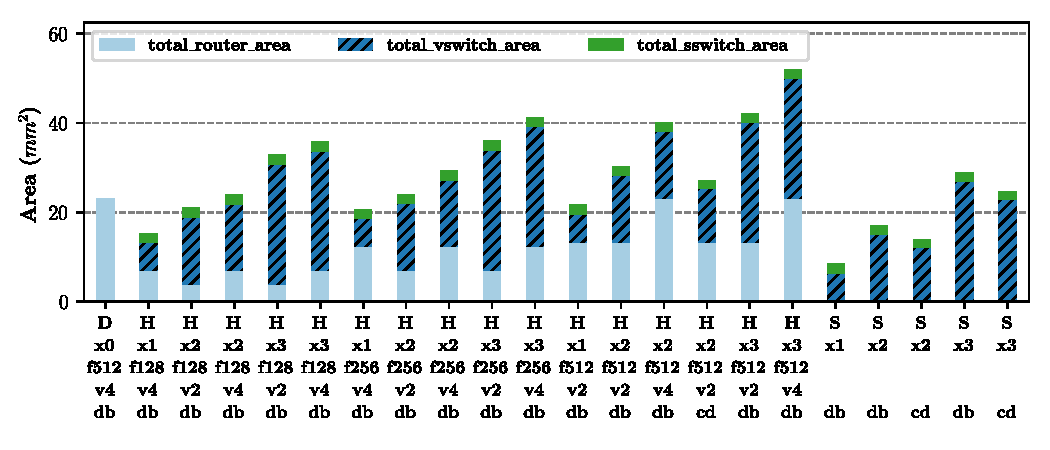
\includegraphics[width=\columnwidth]{figs/area.pdf}
%\caption{Area breakdown of network architectures}\label{fig:area}
%\end{figure}

%In this section, we evaluate the proposed network architecture design points from Section~\ref{sec:network}, summarized in Table~\ref{tab:net_dse}.
%Pure dynamic networks are represented with $D{\dash}v0{\dash}s0$, indicating no static links in the network. 
%Pure static networks are prefixed with $v\#{\dash}s\#$, where the $\#$ are number of
%scalar and vector links between switches. Hybrid networks are shown as $D{\dash}v\#{\dash}s\#$.
%Figure~\ref{fig:area_vc} (a) shows the number of VCs required to map each application for architectures containing a dynamic network. 
%%The maximum number of VCs required across all applications is the number of VCs we use to account for area. 
%When computing area for each configuration, we use the maximum number of VCs required to map any application.
%For application in hybrid network with no VCs, all traffic is mapped onto the static network.

%Figure~\ref{fig:area_vc} (b) shows the area breakdown of the architecture. 
%For $D{\dash}v0{\dash}s0$, all links are routed through the dynamic network, resulting in heavy congestion and a large VC requirement. 
%Consequently, the large number of VCs directly contribute to the large router area. 
%All the other dynamic configurations only need 2 VCs to avoid deadlock. 
%The network area contributes only a small fraction of the overall area, but using a dynamic network with a smaller flit width saves router area roughly linearly.
%%The hybrid network $D{\dash}v1{\dash}s4-f512, and D{\dash}v2{\dash}s4-f512$ has slightly larger area than their equivalent bandwidth counterpart design point in static network $v2{\dash}s4$ and $v3{\dash}s4$ due to the overhead on dynamic routing and buffering. 

%Figure~\ref{fig:slow_down} (a) shows the performance degradation normalized to the ideal network with infinite buffers; all the other design points have an end-point buffer with depth 4 inside the CUs.
%We found that for memory bandwidth bound applications, the performance is roughly the same across all design points, mostly due to the low CU utilization and lack of congestion. 
%Although BlackScholes is DRAM bandwidth bound, the inner loop partition introduces lots of CUs communicating their temporary results. 
%The slow-down with BlackScholes with static network compared to ideal network is due to the pipeline bubbles introduced by VB partitioning as explained in Section \ref{sec:network}. 

%Overall, the hybrid network with the $v1$ static network has a slowdown of less than 2x overall, while the hybrid network with $v2$ has static-equivalent performance.

%The static network with credit-based flow control suffers from insufficient end-point buffers for most applications, resulting in poor performance. 
%The slowdown in dynamic and hybrid networks is mostly due to the high-throughput broadcasts and congestion. 
%Figure~\ref{fig:slow_down} (b) shows the slowdown normalized to total area. 
%Since the network only takes a small fraction of the chip area, the trends is similar to performance. 

%Figure~\ref{fig:slow_down}(c) shows the network energy normalized to $v2{\dash}s4$. 
%The pure dynamic network consumes the most energy because of the amount of buffers and the router's inherently higher per-flit energy. 
%Breaking down the hybrid network energy, we can see that vast majority of communication is mapped to the static network. 
%There is a small gap between energy on $v2{\dash}s4$ and $D{\dash}v2{\dash}s4$, where the hybrid consumes less energy, even though all traffic is mapped onto the static network. 
%Another outlier on LeNet $D{\dash}v2{\dash}s4$ consumes more energy then $v2{\dash}s4{\dash}db$ is likely introduced by randomness from the iterative placer. 
%These are discrepancies introduced by different placements having different distances between nodes.
%It is also important to note hat the overprovisioned static capacity has a high (31\%) mean energy cost, even though it is not being used.
%%This is due to a limitation in current implementation that pure static networks are placed and routed with only back tracking placer, while the hybrid is also using the iterative placer. 
%%As a result, we found better mapping on hybrid network which reduce the hop distance on links, which is not essential for slowdown but directly translates into energy. 
%%However, in theory we should be able to use both algorithm on all design points. 

%In Figure~\ref{fig:slow_down} (d), we show the normalized power. 
%Here, design points with large slowdown naturally have lower power, such as $v3{\dash}s4{\dash}cd$. 
%However, we also show that the network is consuming only a very small portion of the power compared with the compute tiles. 
%The network only consumes around 0--3 W of energy compared to the theoretical peak Plasticine power of 49W.
%Therefore, among the metrics of performance, area, and power, performance is the most important metric to measure the network architectures. 

%%
%%This allows it to be stored in the smaller buffers without any translation logic, and does not result in a loss of throughput (the throughput would be limited regardless at the non-priority VC).
%%Because the priority VC is considered in route scoring, the placer is able to ensure that less than 1\% of traffic in the worst app (XXX) traverses non-priority VCs.
%%This scheme results in a XXX\% lower network area, with a geometric mean slowdown of XXX\% (worst XXX\%).

  \chapter{Related Work} \label{sec:related}

\section{Compiler}
\paragraph{Streaming Dataflow IRs}
Although many works claim to emit efficient and information-rich dataflow IRs for the downstream compilers, 
very few of them can capture the high-level parallel patterns and implementation details that are critical 
to RDA mappings. 
For example, TensorFlow \cite{tensorflow} emits dataflow IR composed of tensor operations. 
However, its IR lacks information on the parallel patterns within these operations. 
In contrast, most of 
the streaming languages \cite{streamit, synaid, maxj} are not able to extract nested loop-level parallelism 
from modern data-intensive applications. 
For example, StreamIt \cite{streamit}, a language tailored for streaming computing, also adopts distributed 
control as in \name{}. 
However, it lacks the necessary language features to describe deeply and irregularly nested loops that are 
common in modern data-intensive applications.

%\paragraph{Hardware Architectures}
%Spatial reconfigurable accelerators (\eg, Dyser~\cite{dyser} and Tartan~\cite{tartan}) have only one-level of hierarchy.
%Hence, such accelerators' performance can be bottlenecked by their limited interconnect bandwidth and power budget.
%Sparse Processing Unit (SPU)~\cite{sparseaccel} can sustain higher interconnect bandwidth by introducing on-chip hierarchy; however, it lacks support for polyhedral memory banking~\cite{poly_cong}, a pivotal optimization to achieve massive parallel accesses to on-chip memory. Plasticine~\cite{plasticine} provides us with the desired architecture features; however, its compiler lacks the necessary components to support efficient streaming execution. Given that Plasticine resembles many key features of the RDA model, we target Plasticine with \name{}.

\paragraph{Machine Learning Compilers}
\begin{outline}
\1 TensorFlow
\1 Theano: A Python framework for fast computation of mathematical expressions.
\1 Cognitive computing programming paradigm: a corelet language for composing networks of neurosynaptic
cores. I
\cite{onnc}
\end{outline}

Library approach
\begin{outline}
\1 Mxnet: A flexible and efficient machine learning library for heterogeneous distributed systems
\1 Anintroductiontocomputational networks and the computational network toolkit
\1 Neural Network Transformation and Co-design under Neuromorphic Hardware Constraints.
\1 Caffe: Convolu- tional architecture for fast feature embedding.
\1 Cambricon: An instruction set architecture for neu- ral networks.
\1 Tangram: Optimized Coarse-Grained Dataflow for Scalable NN Accelerators
\end{outline}

Kernel-specific loop optimization
\begin{outline}
\1 Tangram: Optimized Coarse-Grained Dataflow for Scalable NN Accelerators
\end{outline}

\paragraph{ML Accelerators}
\begin{outline}
%% Dataflow accelerators
\1 A runtime reconfigurable dataflow processor for vision
\1 Tangram: Optimized Coarse-Grained Dataflow for Scalable NN Accelerators
\1 %% domain specific loop fushion inter change
\1 Truenorth: Design and tool flow of a 65 mw 1 million neuron programmable neurosynaptic chip. from
IBM
\1 Memristive Boltzmann machine: A hardware accelerator for combinatorial optimization and deep
learning. 
\1 Scalable hierarchical network-on- chip architecture for spiking neural network hardware
implementations. 
\1 Diannao: A small-footprint high-throughput accel- erator for ubiquitous machine-learning.
\1 Pudiannao: A polyvalent machine learning accelerator. In ACM SIGARCH Computer Architecture News, Vol.
43. ACM, 369–381.
\1 Eyeriss: An energy- efficient reconfigurable accelerator for deep convolutional neural networks. I
\1 EIE: efficient inference engine on compressed deep neural network.
\1 Design and evolution of modular neural network architectures
\1 In-Datacenter Performance Analysis of a Tensor Processing Unit. 
\1 RENO: A high- efficient reconfigurable neuromorphic computing accelerator design.
\1 Convolution engine: balancing efficiency \& flexibility in specialized computing.
\1 Minerva: Enabling low-power, highly-accurate deep neural network acceler- ators. 
\1 DNPU: An 8.1TOPS/W Reconfigurable CNN-RNN Processor for General Purpose Deep Neu- ral Networks. 
\1 C-Brain: A deep learning accelerator that tames the diversity of CNNs through adaptive data-level
\1 parallelization. 
\end{outline}

\paragraph{Spatial Compilers}
Most previous works \cite{nowatzki, spatial-computation} only consider allocating resources at the same level. 
\name{} takes a more general assumption by co-allocating resources at multiple levels of an accelerator's hierarchy.

%The Plasticine compiler~\cite{plasticine} is similar to \name{} that it also uses a token-based control protocol.
%However, it performs worse than \name{} due to the following reasons.
%First, the Plasticine compiler allocates VBs for every level of Spatial's (a high-level language) control hierarchy. 
%The communication between parent and child controllers lead to both communication hotspots around the parent, and bubbles before entering a steady-state of the loop iterations. 
%Second, the Plasticine compiler assigns a single memory PB for each logical memory in the Spatial program. 
%Hence, it could not handle the case where a logical memory exceeds the capacity or bank limits of the physical PBs.
%Third, the Plasticine compiler only supports polyhedral memory partitioning at the first dimension of the on-chip memory. 
%Hence, its applicability to data-intensive applications with high-dimension tensor algebra is questionable.
%Last, compared to \name{}'s separate allocation and assignment phases described in
%\Cref{sec:control} and \Cref{sec:resalloc},
%the Plasticine compiler allocates one VB for a specific type of PB and underutilizes resources within PBs.

\section{On-Chip Network}

Multiple decades of research have resulted in a rich body of literature, both in CGRAs~\cite{cgraSurvey1, cgraSurvey2} and on-chip networks~\cite{ocn-synthesis}. We discuss relevant prior work under the following categories:
\subsection{Tiled Processor Interconnects} Architectures such as Raw~\cite{raw} and Tile~\cite{tile} use scalar operand networks~\cite{son}, which combine static and dynamic networks. Raw has one static and two dynamic interconnects: the static interconnect is used to route normal operand traffic, one dynamic network is used to route runtime-dependent values which could not be routed on the static network, and the second dynamic network is used for cache misses and other exceptions. Deadlock avoidance is guaranteed only in the second dynamic network, which is used to recover from deadlocks in the first dynamic network. However, as described in Section~\ref{sec:intro}, wider buses and larger flit sizes create scalability issues with two dynamic networks, including higher area and power. In addition, our static VC allocation scheme ensures deadlock freedom in our single dynamic network, obviating the need for deadlock recovery.
The dynamic Raw network also does not preserve operand ordering, requiring an operand reordering mechanism at every tile.

TRIPS~\cite{trips} is a tiled dataflow architecture with dynamic execution. TRIPS does not have a static interconnect, but contains two dynamic networks~\cite{trips-network}: an operand network  to route operands between tiles, and an on-chip network  to communicate with cache banks. Wavescalar~\cite{wavescalar} is another tiled dataflow architecture with four levels of hierarchy, connected by dynamic interconnects that vary in topology and bandwidth at each level. The Polymorphic Pipeline Array~\cite{ppa} is a tiled architecture built to target mobile multimedia applications. While compute resources are either statically or dynamically provisioned via hardware virtualization support, communication uses a dynamic scalar operand network.

\subsection{CGRA Interconnects}
Many previously proposed CGRAs use a word-level static interconnect, which has better compute density than bit-based routing~\cite{bus-fpga}. CGRAs such as HRL~\cite{hrl}, DySER~\cite{dyser}, and Elastic CGRAs~\cite{elasticCGRAs} commonly employ two static interconnects: a word-level interconnect to route data and a bit-level interconnect to route control signals.
Several works have also proposed a statically scheduled interconnect~\cite{van2009static, dimitroulakos2006exploring, wave} using a modulo schedule. While this approach is effective for inner loops with predictable latencies and fixed initiation intervals, variable latency operations and hierarchical loop nests add scheduling complexity that prevents a single modulo schedule. HyCube~\cite{hycube} has a similar statically scheduled network, with the ability to bypass intermediate switches in the same cycle. This allows operands to travel multiple hops in a single cycle, but creates long wires and combinational paths and adversely affects the clock period and scalability.
%However, applications with a hierarchical nesting of loops provide two poor options to arrive a single modulo schedule: the II can be extended to cover the entirety of the innermost loop, or the outer loop can have resources reserved in the inner loop schedule.
%The first option is frequently not realistic because scheduled hardware has a hard cap on the II, and loops can be of arbitrary length.
%If outer loops have resources reserved in the inner loop schedule, then the schedule will become congested with reserved, but infrequently used, resources.
\subsection{Design Space Studies} Several prior studies focus on tradeoffs with various network topologies, but do not characterize or quantify the role of dynamism in interconnects.
The Raw design space study~\cite{dse-raw} uses an analytical model for applications as well as architectural resources to perform a sensitivity analysis of compute and memory resources focused on area, power, and performance, without varying the interconnect. The ADRES design space study~\cite{dse-adres} focuses on area and energy tradeoffs with different network topologies with the ADRES~\cite{adres} architecture, where all topologies use a fully static interconnect. KressArray Xplorer~\cite{dse-kressarray} similarly explores topology tradeoffs with the KressArray~\cite{kress} architecture. Other studies explore topologies for mesh-based CGRAs~\cite{dse-date} and more general CGRAs supporting resource sharing~\cite{dse-tvlsi}. Other tools like Sunmap~\cite{sunmap} allow end users to construct and explore various topologies.

\subsection{Compiler Driven NoCs (WIP)}
Other prior works have used compiler techniques to optimize various facets of NoCs.
Some studies have explored statically allocating virtual channels~\cite{staticVC-isca, staticVC-nocs} to multiple concurrent flows to mitigate head-of-line blocking. These studies propose an approach to derive deadlock-free allocations based on the turn model~\cite{turnModel}. While our approach also statically allocates VCs, our method to guarantee deadlock freedom differs from the aforementioned study as it does not rely on the turn model.
Ozturk et al. \cite{ozturk2010compiler} propose a scheme to increase the reliability of NoCs for chip multiprocessors by sending packets over multiple links.
Their approach uses integer linear programming to balance the total number of links activated (an energy-based metric) against the amount of packet duplication (reliability).
Ababei et al. \cite{ababei2011energy} use a static placement algorithm and an estimate of reliability to attempt to guide placement decisions for NoCs.
Kapre et al. \cite{kapre2011noc} develop a workflow to map applications to CGRAs using several transformations, including efficient multicast routing and node splitting, but do not consider optimizations such as non-minimal routing.

%Our approach provides an extension of these techniques by using a ``closed-loop'' iterative process.
%Instead of doing each step (placement, routing, deadlock avoidance) sequentially, we are able to use heuristics to quantify the impact that each step has on the badness of the overall design.
%For example, this allows us to fix routing pathologies by re-placement, because we can identify the specific placement decisions that led to the poor set of routes.


% Ignore arch for now; we assume arch

% \paragraph{Plasticine Compiler}
% The Plasticine compiler described in the original paper also uses a token-based control protocal.
% However, the Plasticine compiler still allocates VB for each level of the controller hierarchy in Spatial
% and pass tokens between the parent and child controllers, which creates communication hot-spot around the
% parant controller and suffers from bubble during warmup phase of the loop iteartions.
% \yz{Rephrase this}
% In addition, their compiler assigns a single memory PB to each logical memory in the program; 
% the compiler cannot handle logical memory exceeding capacity or bank limit of the physical PBs.
% The simple strided banking scheme also disallows parallelized access on multiple dimension of the memory,
% which can greatly limits the application design space.
% Finally, unlike spaerate allocation and assignment phases described in \Cref{sec:alloc} and \Cref{sec:pruning},
% they allocate a VB for a specific type of PB, which under under utilizes resource whin PBs.


% \gist{
% CGRA: \\
% \cite{tartan} \\
% Imperative to Spatial Architectures: \\
% \cite{synaid}: 
% \begin{outline}
% \1 Target green array. Tiles of stack based 18-bit processors. Small local memory per
% core.
% \1 Small benchmarks: trigonometric, FFT, bithack, etc..
% \end{outline}
% \cite{zaidi}
% His thesis:\\
% \url{https://www.cl.cam.ac.uk/techreports/UCAM-CL-TR-870.pdf} \\
% Targeting FPGA. We probably don't want to cite this guy.

% Partitioning: \\
% \cite{nowatzki} - Partitioning data flow graph using ISL \\

% Summary:
% Looks like we are not the first one trying to map imperative language to spatial architecture. But there are still major differences.
% Some of the work is mapping to FPGAs, similar to high-level synthesis tools.
% Many of the other works like \cite{zaidi} only focus on the data-flow graph and do not handle memory accesses. Although we both trying to support imperative language on spatial accelerator, our focus is never to accelerate control heavy code on the accelerator, but rather to target data intensive application with more flexibility.

% \cite{synaid} is actually very relevant but the architecture is at a much smaller scale. It does have distributed on-chip memory but their memory is a stack used to store program for processors. None of the prior work has consider using distributed memory to compose logically single memory with strong-consistency and coherence. Another major difference is that these architecture does not have global network and DRAM that introduces variable latency. 
% So this changes how the application is mapped onto the accelerator. Our approach is completely distributed streaming approach while they tends to use statically scheduled approach.
% Finally the applications are very different. Most of their applications are very small kernels or image/audio encoding/decoding. Our benchmarks has a mix of full ML models + graph + others
% }

% Maybe related \cite{sparseaccel}

% Triggered Instruction \cite{ti}
% Tartan\cite{tartan}

% \gist{
% 	\begin{itemize}
% 		\item Plasticine compiler: \cite{plasticine}
% 		\item Tartan: \cite{tartan} Single op partitions w/ handshaking, direct template translation.
% 		\item Zaidi Thesis: \cite{zaidi} Conversion to bluespec, also uses token-based control. No partitioning / merging.
% 		\item Partitioning: \cite{nowatzki} Solver-based partitioning, very small arrays (4x4 dyser, etc.), with statically known delays and single-op partitions. Does not handle merging.
% 		\item SparseAccel: \cite{sparseaccel}\ Architecture paper, basically nothing about compilers.  (NR)
% 		\item streamit for RAW: \cite{streamit} No memory consistency due to pure stream structure, fine grained arch. Mesh of processors.
% 		\item Triggered Instructions \cite{ti} Fine grained processor architecture, with caches. (Micro paper: manual mapping, assembly, NR)
% 		\item Chlorophyll: \cite{synaid} Maps subset of C to GreenArrays (small spatial stack-processor architecture). Distinct Non-distributed arrays vs distributed arrays, optional partition annotations, static for loops (unrestricted while), uses Rosette backend solver (branch and bound, SA, Ant, Tabu Search, picked Simulated Annealing). Actual generation is synthesis based.
% 		\item Spatial computation \cite{spatial-computation} Maps ANSI C to Verilog, handshake + token based execution with speculative execution. Uses crossbar network for memory (although we assume pre-banked memory). Fine grained control, uses Pegasus for memory dependence graph and tokens for synchronization. Does not address partitioning / merging.
% 	\end{itemize}
% }

  \chapter{Conclusions (WIP)} \label{sec:conclusion}

Reconfigurable dataflow accelerators (RDAs) are a promising class of spatial accelerators, which deliver higher performance-to-resource efficiency than conventional process architectures while capturing a large application space.
However, to sustain these benefits as RDAs get larger, the software stack must address the challenges of (a) distributed control / correctness and (b) efficient resource allocation.

We address these challenges by proposing a distributed asynchronous control scheme and a program decomposition method. 
We develop a compiler, \name{}, that constructs a virtual block dataflow graph (VBDFG) from a program specification and generates a minimal set of peer-to-peer synchronizations, which allow fine-grained parallelization factors that would otherwise incur large communication overheads.
Furthermore, operations on VBDFG are decomposed and assigned to a heterogenous collections of physical blocks (PBs). 
Lastly, we implement these techniques and through evaluations show that \name{} achieves a speedup of 4x over a Tesla V100 GPU.
We hope that the approach and implementation presented in this work will help scale modern RDAs add a steady pace..

We show that the best network design depends on both applications and the underlying accelerator architecture.
Network performance correlates strongly with bandwidth for streaming accelerators, and scaling raw bandwidth is more area- and energy-efficient with a static network.
We show that the application mapping can be optimized to move less data by using a dynamic network as a fallback from a high-bandwidth static network.
%this contributes a 6.9x average performance per area and 2.3x average energy-efficiency improvement for a static-dynamic hybrid network.
This static-dynamic hybrid network provides a 1.8x energy-efficiency and
2.8x performance advantage over the purely static and purely dynamic networks, respectively.
  %Furthermore, we show that spatial architectures require larger switches as programs get bigger, imposing super-linear scaling of network size with chip area.



  \section{Acknowledgement}

We appreciate the anonymous reviewers for their feedback.
We thank Matthew Feldman for compiler support
  and his constructive suggestions on the manuscript of this paper,
  and Raghu Prabhakar for providing insights and
  feedback on the architecture section of this paper.
We also thank Google for the cloud credits.
This material is based on research sponsored by Air Force Research Laboratory (AFRL) and Defense
Advanced Research Projects Agency (DARPA) under agreement number FA8650-18-2-7865. The U.S.
Government is authorized to reproduce and distribute reprints for Governmental purposes
notwithstanding any copyright notation thereon. The views and conclusions contained herein are those
of the authors and should not be interpreted as necessarily representing the official policies or
endorsements, either expressed or implied, of Air Force Research Laboratory (AFRL) and Defense
Advanced Research Projects Agency (DARPA) or the U.S. Government.
This research is also supported in part by affiliate members and other supporters of the
Stanford DAWN project - Ant Financial, Facebook, Google, Infosys, Intel, Microsoft, NEC, Teradata,
SAP and VMware.

  \bibliographystyle{sysml2019}
  \bibliography{references}
  %%%%%%%%%%%%%%%%%%%%%%%%%%%%%%%%%%%%%%%%%%%%%%%%%%%%%%%%%%%%%%%%%%%%%%%%%%%%%%%
  %%%%%%%%%%%%%%%%%%%%%%%%%%%%%%%%%%%%%%%%%%%%%%%%%%%%%%%%%%%%%%%%%%%%%%%%%%%%%%%
\end{document}
